% Options for packages loaded elsewhere
\PassOptionsToPackage{unicode}{hyperref}
\PassOptionsToPackage{hyphens}{url}
%
\documentclass[
]{book}
\usepackage{amsmath,amssymb}
\usepackage{iftex}
\ifPDFTeX
  \usepackage[T1]{fontenc}
  \usepackage[utf8]{inputenc}
  \usepackage{textcomp} % provide euro and other symbols
\else % if luatex or xetex
  \usepackage{unicode-math} % this also loads fontspec
  \defaultfontfeatures{Scale=MatchLowercase}
  \defaultfontfeatures[\rmfamily]{Ligatures=TeX,Scale=1}
\fi
\usepackage{lmodern}
\ifPDFTeX\else
  % xetex/luatex font selection
\fi
% Use upquote if available, for straight quotes in verbatim environments
\IfFileExists{upquote.sty}{\usepackage{upquote}}{}
\IfFileExists{microtype.sty}{% use microtype if available
  \usepackage[]{microtype}
  \UseMicrotypeSet[protrusion]{basicmath} % disable protrusion for tt fonts
}{}
\makeatletter
\@ifundefined{KOMAClassName}{% if non-KOMA class
  \IfFileExists{parskip.sty}{%
    \usepackage{parskip}
  }{% else
    \setlength{\parindent}{0pt}
    \setlength{\parskip}{6pt plus 2pt minus 1pt}}
}{% if KOMA class
  \KOMAoptions{parskip=half}}
\makeatother
\usepackage{xcolor}
\usepackage{color}
\usepackage{fancyvrb}
\newcommand{\VerbBar}{|}
\newcommand{\VERB}{\Verb[commandchars=\\\{\}]}
\DefineVerbatimEnvironment{Highlighting}{Verbatim}{commandchars=\\\{\}}
% Add ',fontsize=\small' for more characters per line
\usepackage{framed}
\definecolor{shadecolor}{RGB}{248,248,248}
\newenvironment{Shaded}{\begin{snugshade}}{\end{snugshade}}
\newcommand{\AlertTok}[1]{\textcolor[rgb]{0.94,0.16,0.16}{#1}}
\newcommand{\AnnotationTok}[1]{\textcolor[rgb]{0.56,0.35,0.01}{\textbf{\textit{#1}}}}
\newcommand{\AttributeTok}[1]{\textcolor[rgb]{0.13,0.29,0.53}{#1}}
\newcommand{\BaseNTok}[1]{\textcolor[rgb]{0.00,0.00,0.81}{#1}}
\newcommand{\BuiltInTok}[1]{#1}
\newcommand{\CharTok}[1]{\textcolor[rgb]{0.31,0.60,0.02}{#1}}
\newcommand{\CommentTok}[1]{\textcolor[rgb]{0.56,0.35,0.01}{\textit{#1}}}
\newcommand{\CommentVarTok}[1]{\textcolor[rgb]{0.56,0.35,0.01}{\textbf{\textit{#1}}}}
\newcommand{\ConstantTok}[1]{\textcolor[rgb]{0.56,0.35,0.01}{#1}}
\newcommand{\ControlFlowTok}[1]{\textcolor[rgb]{0.13,0.29,0.53}{\textbf{#1}}}
\newcommand{\DataTypeTok}[1]{\textcolor[rgb]{0.13,0.29,0.53}{#1}}
\newcommand{\DecValTok}[1]{\textcolor[rgb]{0.00,0.00,0.81}{#1}}
\newcommand{\DocumentationTok}[1]{\textcolor[rgb]{0.56,0.35,0.01}{\textbf{\textit{#1}}}}
\newcommand{\ErrorTok}[1]{\textcolor[rgb]{0.64,0.00,0.00}{\textbf{#1}}}
\newcommand{\ExtensionTok}[1]{#1}
\newcommand{\FloatTok}[1]{\textcolor[rgb]{0.00,0.00,0.81}{#1}}
\newcommand{\FunctionTok}[1]{\textcolor[rgb]{0.13,0.29,0.53}{\textbf{#1}}}
\newcommand{\ImportTok}[1]{#1}
\newcommand{\InformationTok}[1]{\textcolor[rgb]{0.56,0.35,0.01}{\textbf{\textit{#1}}}}
\newcommand{\KeywordTok}[1]{\textcolor[rgb]{0.13,0.29,0.53}{\textbf{#1}}}
\newcommand{\NormalTok}[1]{#1}
\newcommand{\OperatorTok}[1]{\textcolor[rgb]{0.81,0.36,0.00}{\textbf{#1}}}
\newcommand{\OtherTok}[1]{\textcolor[rgb]{0.56,0.35,0.01}{#1}}
\newcommand{\PreprocessorTok}[1]{\textcolor[rgb]{0.56,0.35,0.01}{\textit{#1}}}
\newcommand{\RegionMarkerTok}[1]{#1}
\newcommand{\SpecialCharTok}[1]{\textcolor[rgb]{0.81,0.36,0.00}{\textbf{#1}}}
\newcommand{\SpecialStringTok}[1]{\textcolor[rgb]{0.31,0.60,0.02}{#1}}
\newcommand{\StringTok}[1]{\textcolor[rgb]{0.31,0.60,0.02}{#1}}
\newcommand{\VariableTok}[1]{\textcolor[rgb]{0.00,0.00,0.00}{#1}}
\newcommand{\VerbatimStringTok}[1]{\textcolor[rgb]{0.31,0.60,0.02}{#1}}
\newcommand{\WarningTok}[1]{\textcolor[rgb]{0.56,0.35,0.01}{\textbf{\textit{#1}}}}
\usepackage{longtable,booktabs,array}
\usepackage{calc} % for calculating minipage widths
% Correct order of tables after \paragraph or \subparagraph
\usepackage{etoolbox}
\makeatletter
\patchcmd\longtable{\par}{\if@noskipsec\mbox{}\fi\par}{}{}
\makeatother
% Allow footnotes in longtable head/foot
\IfFileExists{footnotehyper.sty}{\usepackage{footnotehyper}}{\usepackage{footnote}}
\makesavenoteenv{longtable}
\usepackage{graphicx}
\makeatletter
\def\maxwidth{\ifdim\Gin@nat@width>\linewidth\linewidth\else\Gin@nat@width\fi}
\def\maxheight{\ifdim\Gin@nat@height>\textheight\textheight\else\Gin@nat@height\fi}
\makeatother
% Scale images if necessary, so that they will not overflow the page
% margins by default, and it is still possible to overwrite the defaults
% using explicit options in \includegraphics[width, height, ...]{}
\setkeys{Gin}{width=\maxwidth,height=\maxheight,keepaspectratio}
% Set default figure placement to htbp
\makeatletter
\def\fps@figure{htbp}
\makeatother
\setlength{\emergencystretch}{3em} % prevent overfull lines
\providecommand{\tightlist}{%
  \setlength{\itemsep}{0pt}\setlength{\parskip}{0pt}}
\setcounter{secnumdepth}{5}
\usepackage{booktabs}
\ifLuaTeX
  \usepackage{selnolig}  % disable illegal ligatures
\fi
\usepackage[]{natbib}
\bibliographystyle{plainnat}
\usepackage{bookmark}
\IfFileExists{xurl.sty}{\usepackage{xurl}}{} % add URL line breaks if available
\urlstyle{same}
\hypersetup{
  pdftitle={Tutorials for Tidymass shinyapp},
  hidelinks,
  pdfcreator={LaTeX via pandoc}}

\title{Tutorials for Tidymass shinyapp}
\author{}
\date{\vspace{-2.5em}}

\begin{document}
\maketitle

{
\setcounter{tocdepth}{1}
\tableofcontents
}
\chapter{Installation}\label{installation}

\textbf{tidymass shinyapp} (\url{https://github.com/tidymass/tidymass_shiny}) is a user-friendly web application for \textbf{tidymass} (\url{https://www.tidymass.org/}) that requires little or no programming experience.

The app can only be installed via code now, and we will introduce how to do that step by step in this chapter.

\section{Preparations}\label{preparations}

To begin with, you need to install R and Rstudio, both of which can be free downloaded from official websites.

If you have installed them before, please ensure that R version \textgreater{} 4.1 as tidymass required, ohterwise download and install the \href{https://cran.r-project.org/mirrors.html}{latest version of R}.

\textbf{Install R}

Download \href{https://www.r-project.org/}{R} and install it.

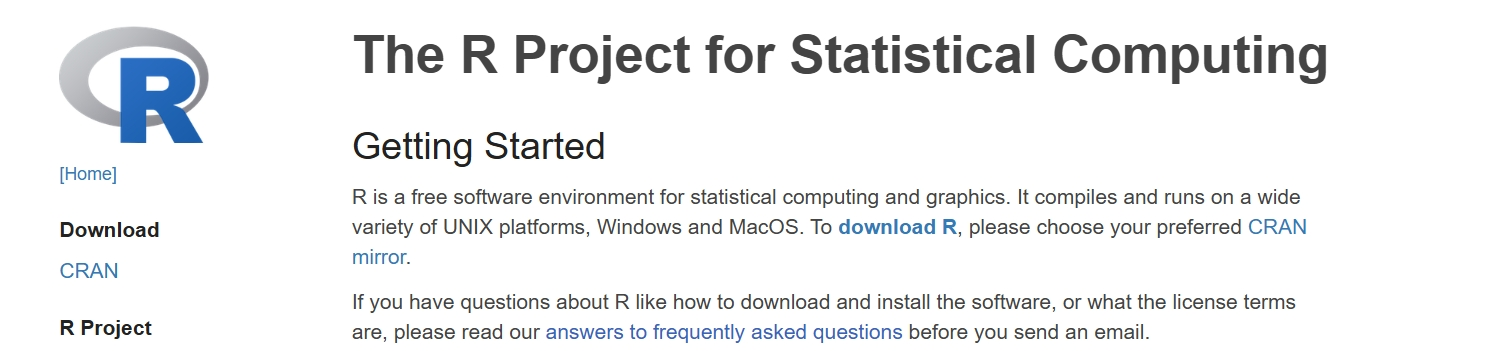
\includegraphics{figures/R_install.png}

\textbf{Install Rstudio}

Download \href{https://posit.co/download/rstudio-desktop/\#download}{Rstudio} and install it.

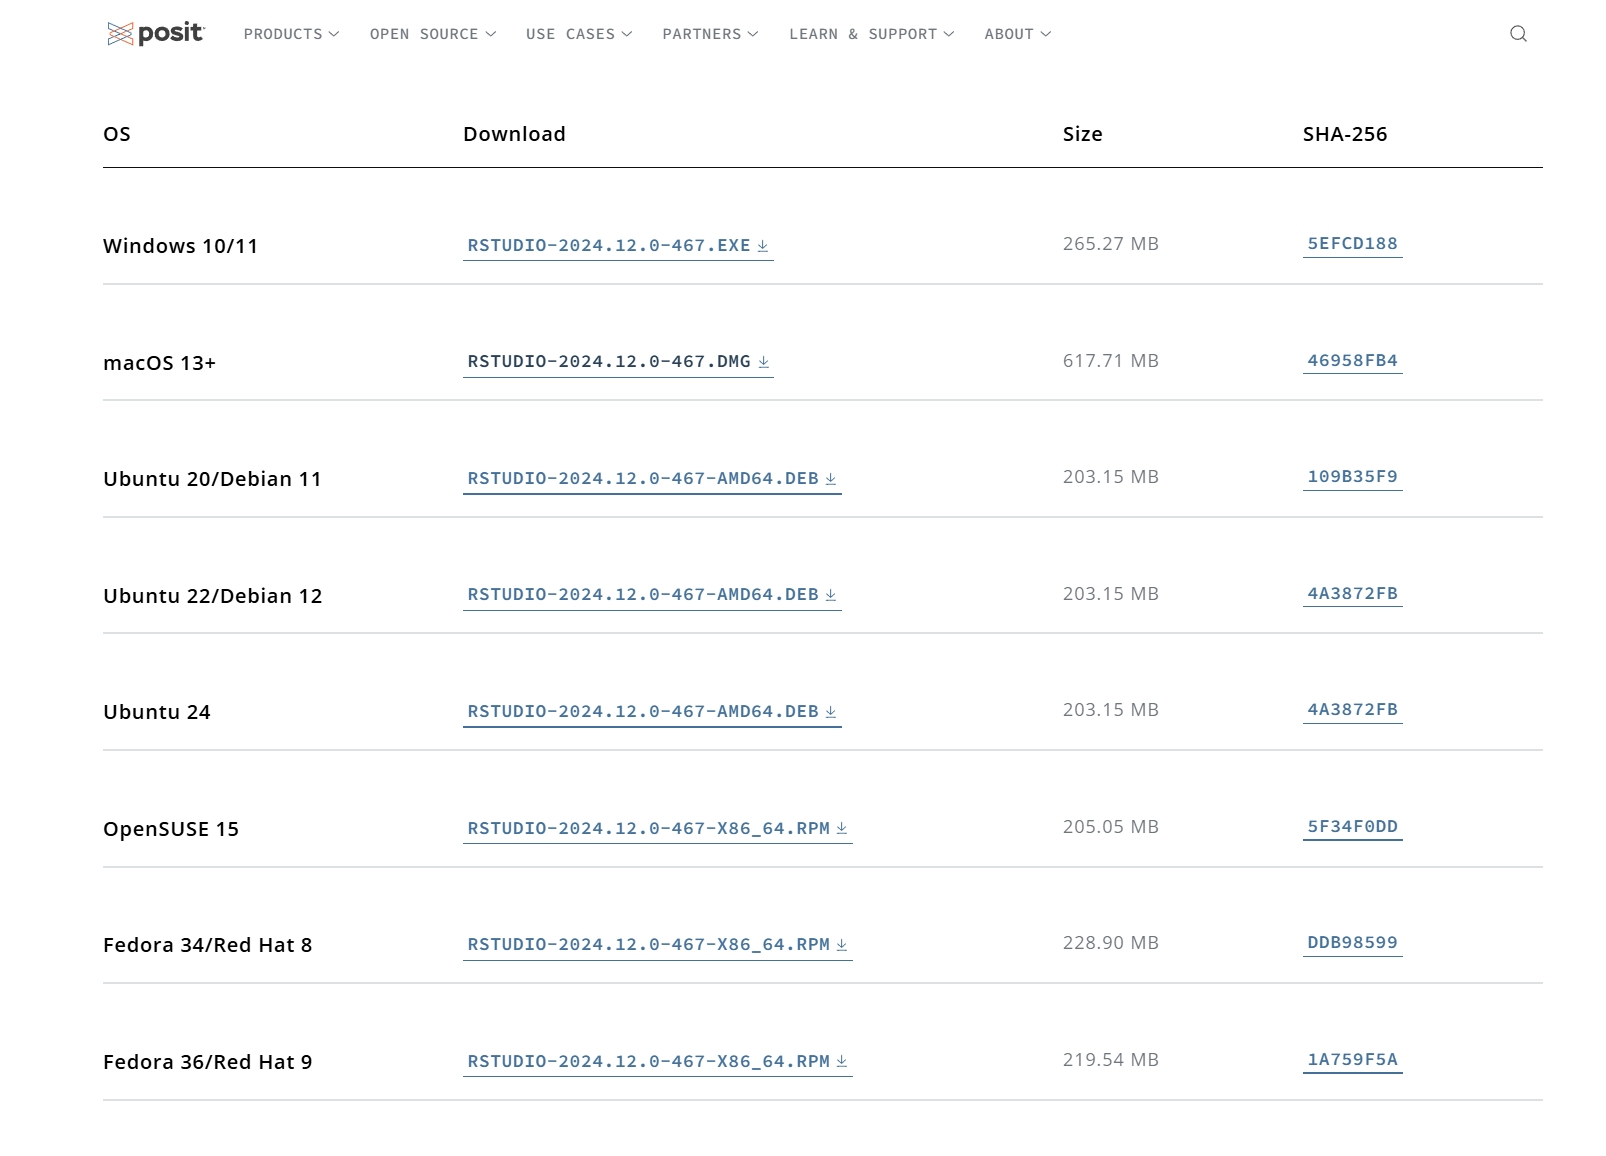
\includegraphics{figures/Rstudio_install.png}

\textbf{Open the Rstudio}

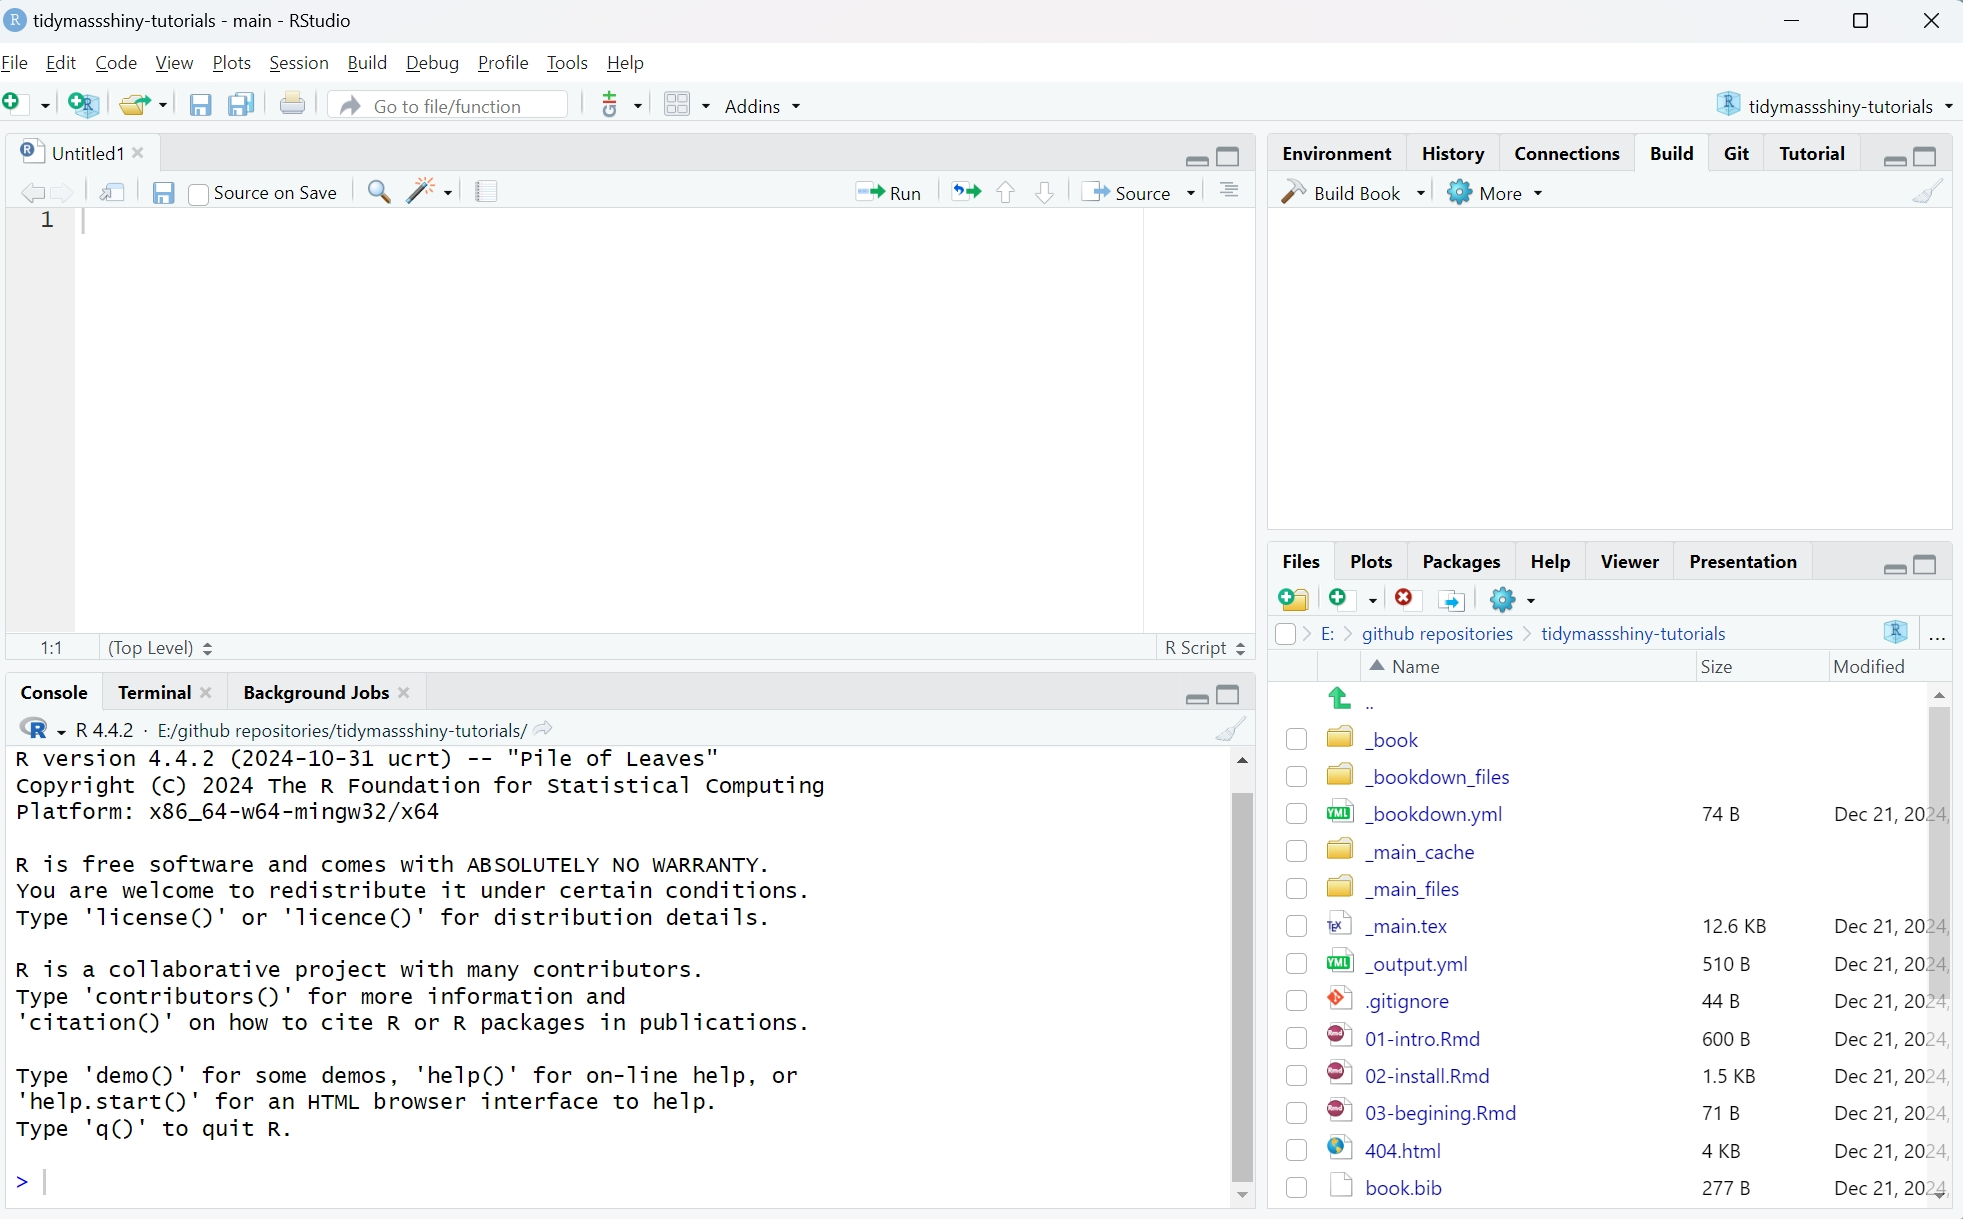
\includegraphics{figures/Rstudio.png}

\textbf{Setting up the suitable Mirror}

You may set up the suitable mirror to accelerate R package downloads.

Click ``Tools'' in the Rstudio, then click ``Global options'' and select ``Packages''. You may select mirror from TUNA Team if you are users from China.

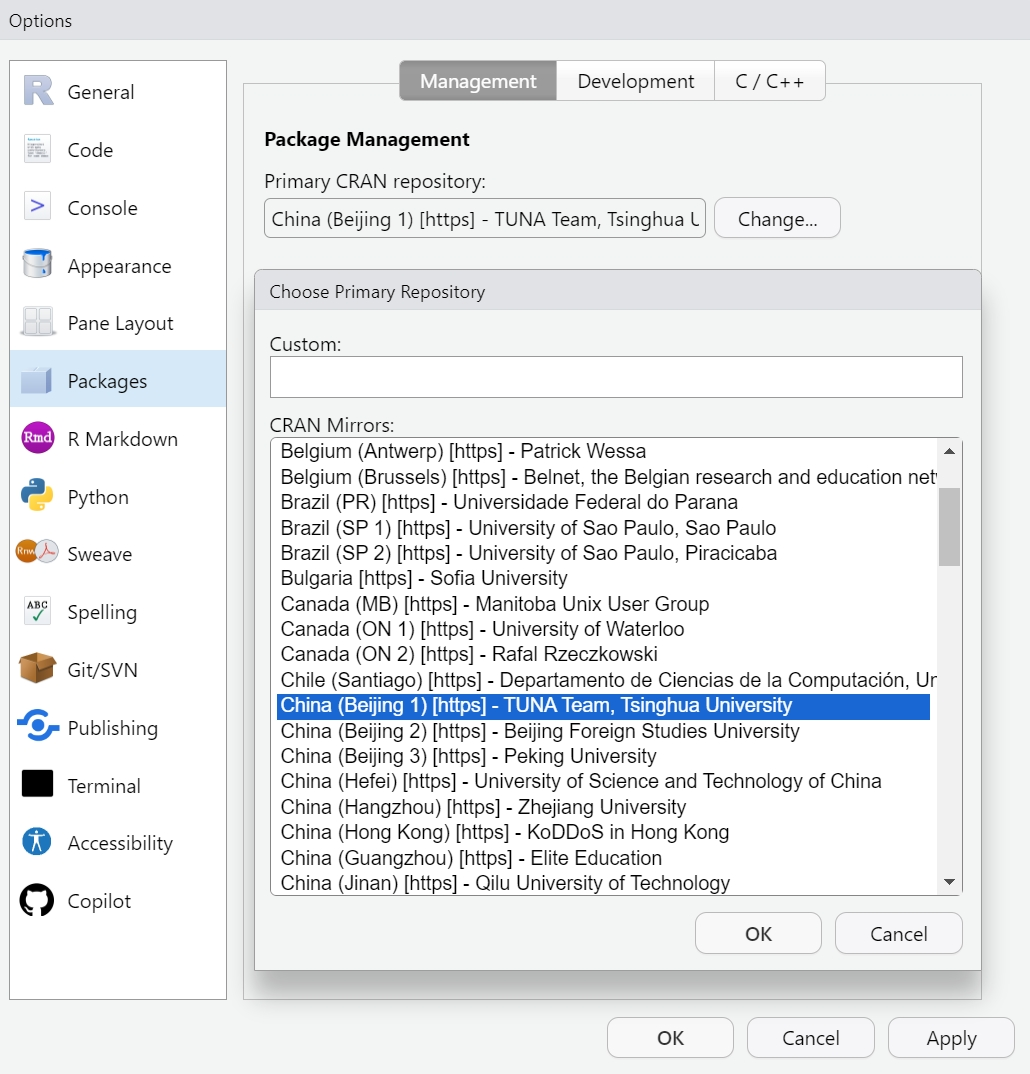
\includegraphics{figures/mirror.png}

\section{Methods to install tidymass shinyapp}\label{methods-to-install-tidymass-shinyapp}

Here we provide three different methods to install tidymass shinyapp: \textbf{R}, \textbf{Docker} and \textbf{Server}.

\textbf{Install with R}

First, you are recommended to install Tidymass with the following code. For more information and help document, please refer to \href{https://www.tidymass.org/}{Tidymass Website}

\begin{Shaded}
\begin{Highlighting}[]
\NormalTok{remotes}\SpecialCharTok{::}\FunctionTok{install\_gitlab}\NormalTok{(}\StringTok{"tidymass/tidymass"}\NormalTok{)}
\end{Highlighting}
\end{Shaded}

Second, install the necessary packages:

\begin{Shaded}
\begin{Highlighting}[]
\ControlFlowTok{if}\NormalTok{ (}\SpecialCharTok{!}\FunctionTok{require}\NormalTok{(}\StringTok{\textquotesingle{}remotes\textquotesingle{}}\NormalTok{)) }\FunctionTok{install.packages}\NormalTok{(}\StringTok{\textquotesingle{}remotes\textquotesingle{}}\NormalTok{);}
\ControlFlowTok{if}\NormalTok{ (}\SpecialCharTok{!}\FunctionTok{require}\NormalTok{(}\StringTok{\textquotesingle{}writexl\textquotesingle{}}\NormalTok{)) }\FunctionTok{install.packages}\NormalTok{(}\StringTok{\textquotesingle{}writexl\textquotesingle{}}\NormalTok{);}
\ControlFlowTok{if}\NormalTok{ (}\SpecialCharTok{!}\FunctionTok{require}\NormalTok{(}\StringTok{\textquotesingle{}Cairo\textquotesingle{}}\NormalTok{)) }\FunctionTok{install.packages}\NormalTok{(}\StringTok{\textquotesingle{}Cairo\textquotesingle{}}\NormalTok{);}
\ControlFlowTok{if}\NormalTok{ (}\SpecialCharTok{!}\FunctionTok{require}\NormalTok{(}\StringTok{\textquotesingle{}tidyverse\textquotesingle{}}\NormalTok{)) }\FunctionTok{install.packages}\NormalTok{(}\StringTok{\textquotesingle{}tidyverse\textquotesingle{}}\NormalTok{);}
\ControlFlowTok{if}\NormalTok{ (}\SpecialCharTok{!}\FunctionTok{require}\NormalTok{(}\StringTok{\textquotesingle{}shinyFiles\textquotesingle{}}\NormalTok{)) remotes}\SpecialCharTok{::}\FunctionTok{install\_github}\NormalTok{(}\StringTok{\textquotesingle{}thomasp85/shinyFiles\textquotesingle{}}\NormalTok{);}
\ControlFlowTok{if}\NormalTok{ (}\SpecialCharTok{!}\FunctionTok{require}\NormalTok{(}\StringTok{\textquotesingle{}shinyWidgets\textquotesingle{}}\NormalTok{)) remotes}\SpecialCharTok{::}\FunctionTok{install\_github}\NormalTok{(}\StringTok{"dreamRs/shinyWidgets"}\NormalTok{);}
\ControlFlowTok{if}\NormalTok{ (}\SpecialCharTok{!}\FunctionTok{require}\NormalTok{(}\StringTok{\textquotesingle{}shiny\textquotesingle{}}\NormalTok{)) }\FunctionTok{install.packages}\NormalTok{(}\StringTok{\textquotesingle{}shiny\textquotesingle{}}\NormalTok{);}
\ControlFlowTok{if}\NormalTok{ (}\SpecialCharTok{!}\FunctionTok{require}\NormalTok{(}\StringTok{\textquotesingle{}shinyalert\textquotesingle{}}\NormalTok{)) }\FunctionTok{install.packages}\NormalTok{(}\StringTok{\textquotesingle{}shinyalert\textquotesingle{}}\NormalTok{);}
\ControlFlowTok{if}\NormalTok{ (}\SpecialCharTok{!}\FunctionTok{require}\NormalTok{(}\StringTok{\textquotesingle{}bsicons\textquotesingle{}}\NormalTok{)) }\FunctionTok{install.packages}\NormalTok{(}\StringTok{\textquotesingle{}bsicons\textquotesingle{}}\NormalTok{);}
\ControlFlowTok{if}\NormalTok{ (}\SpecialCharTok{!}\FunctionTok{require}\NormalTok{(}\StringTok{\textquotesingle{}hexbin\textquotesingle{}}\NormalTok{)) }\FunctionTok{install.packages}\NormalTok{(}\StringTok{\textquotesingle{}hexbin\textquotesingle{}}\NormalTok{);}
\ControlFlowTok{if}\NormalTok{ (}\SpecialCharTok{!}\FunctionTok{require}\NormalTok{(}\StringTok{\textquotesingle{}bslib\textquotesingle{}}\NormalTok{)) }\FunctionTok{install.packages}\NormalTok{(}\StringTok{\textquotesingle{}bslib\textquotesingle{}}\NormalTok{);}
\ControlFlowTok{if}\NormalTok{ (}\SpecialCharTok{!}\FunctionTok{require}\NormalTok{(}\StringTok{\textquotesingle{}plotly\textquotesingle{}}\NormalTok{)) }\FunctionTok{install.packages}\NormalTok{(}\StringTok{\textquotesingle{}plotly\textquotesingle{}}\NormalTok{);}
\ControlFlowTok{if}\NormalTok{ (}\SpecialCharTok{!}\FunctionTok{require}\NormalTok{(}\StringTok{\textquotesingle{}colourpicker\textquotesingle{}}\NormalTok{)) }\FunctionTok{install.packages}\NormalTok{(}\StringTok{\textquotesingle{}colourpicker\textquotesingle{}}\NormalTok{);}
\ControlFlowTok{if}\NormalTok{ (}\SpecialCharTok{!}\FunctionTok{require}\NormalTok{(}\StringTok{\textquotesingle{}plantmdb\textquotesingle{}}\NormalTok{)) remotes}\SpecialCharTok{::}\FunctionTok{install\_github}\NormalTok{(}\StringTok{"xuebinzhang{-}lab/plantmdb"}\NormalTok{)  }\DocumentationTok{\#\# plant metabolomics database. for test use.}
\end{Highlighting}
\end{Shaded}

Finally, install Tidymass shinyapp with the code:

\begin{Shaded}
\begin{Highlighting}[]
\NormalTok{remotes}\SpecialCharTok{::}\FunctionTok{install\_github}\NormalTok{(}\StringTok{\textquotesingle{}tidymass/tidymass\_shiny\textquotesingle{}}\NormalTok{)}
\end{Highlighting}
\end{Shaded}

To start the shiny app, run the code.

\begin{Shaded}
\begin{Highlighting}[]
\FunctionTok{library}\NormalTok{(tidyverse)}
\FunctionTok{library}\NormalTok{(tidymass)}
\FunctionTok{library}\NormalTok{(tidymassshiny)}
\FunctionTok{library}\NormalTok{(plantmdb) }\DocumentationTok{\#\# for test use}
\FunctionTok{run\_tidymass\_shiny}\NormalTok{()}
\end{Highlighting}
\end{Shaded}

You should be able to see:

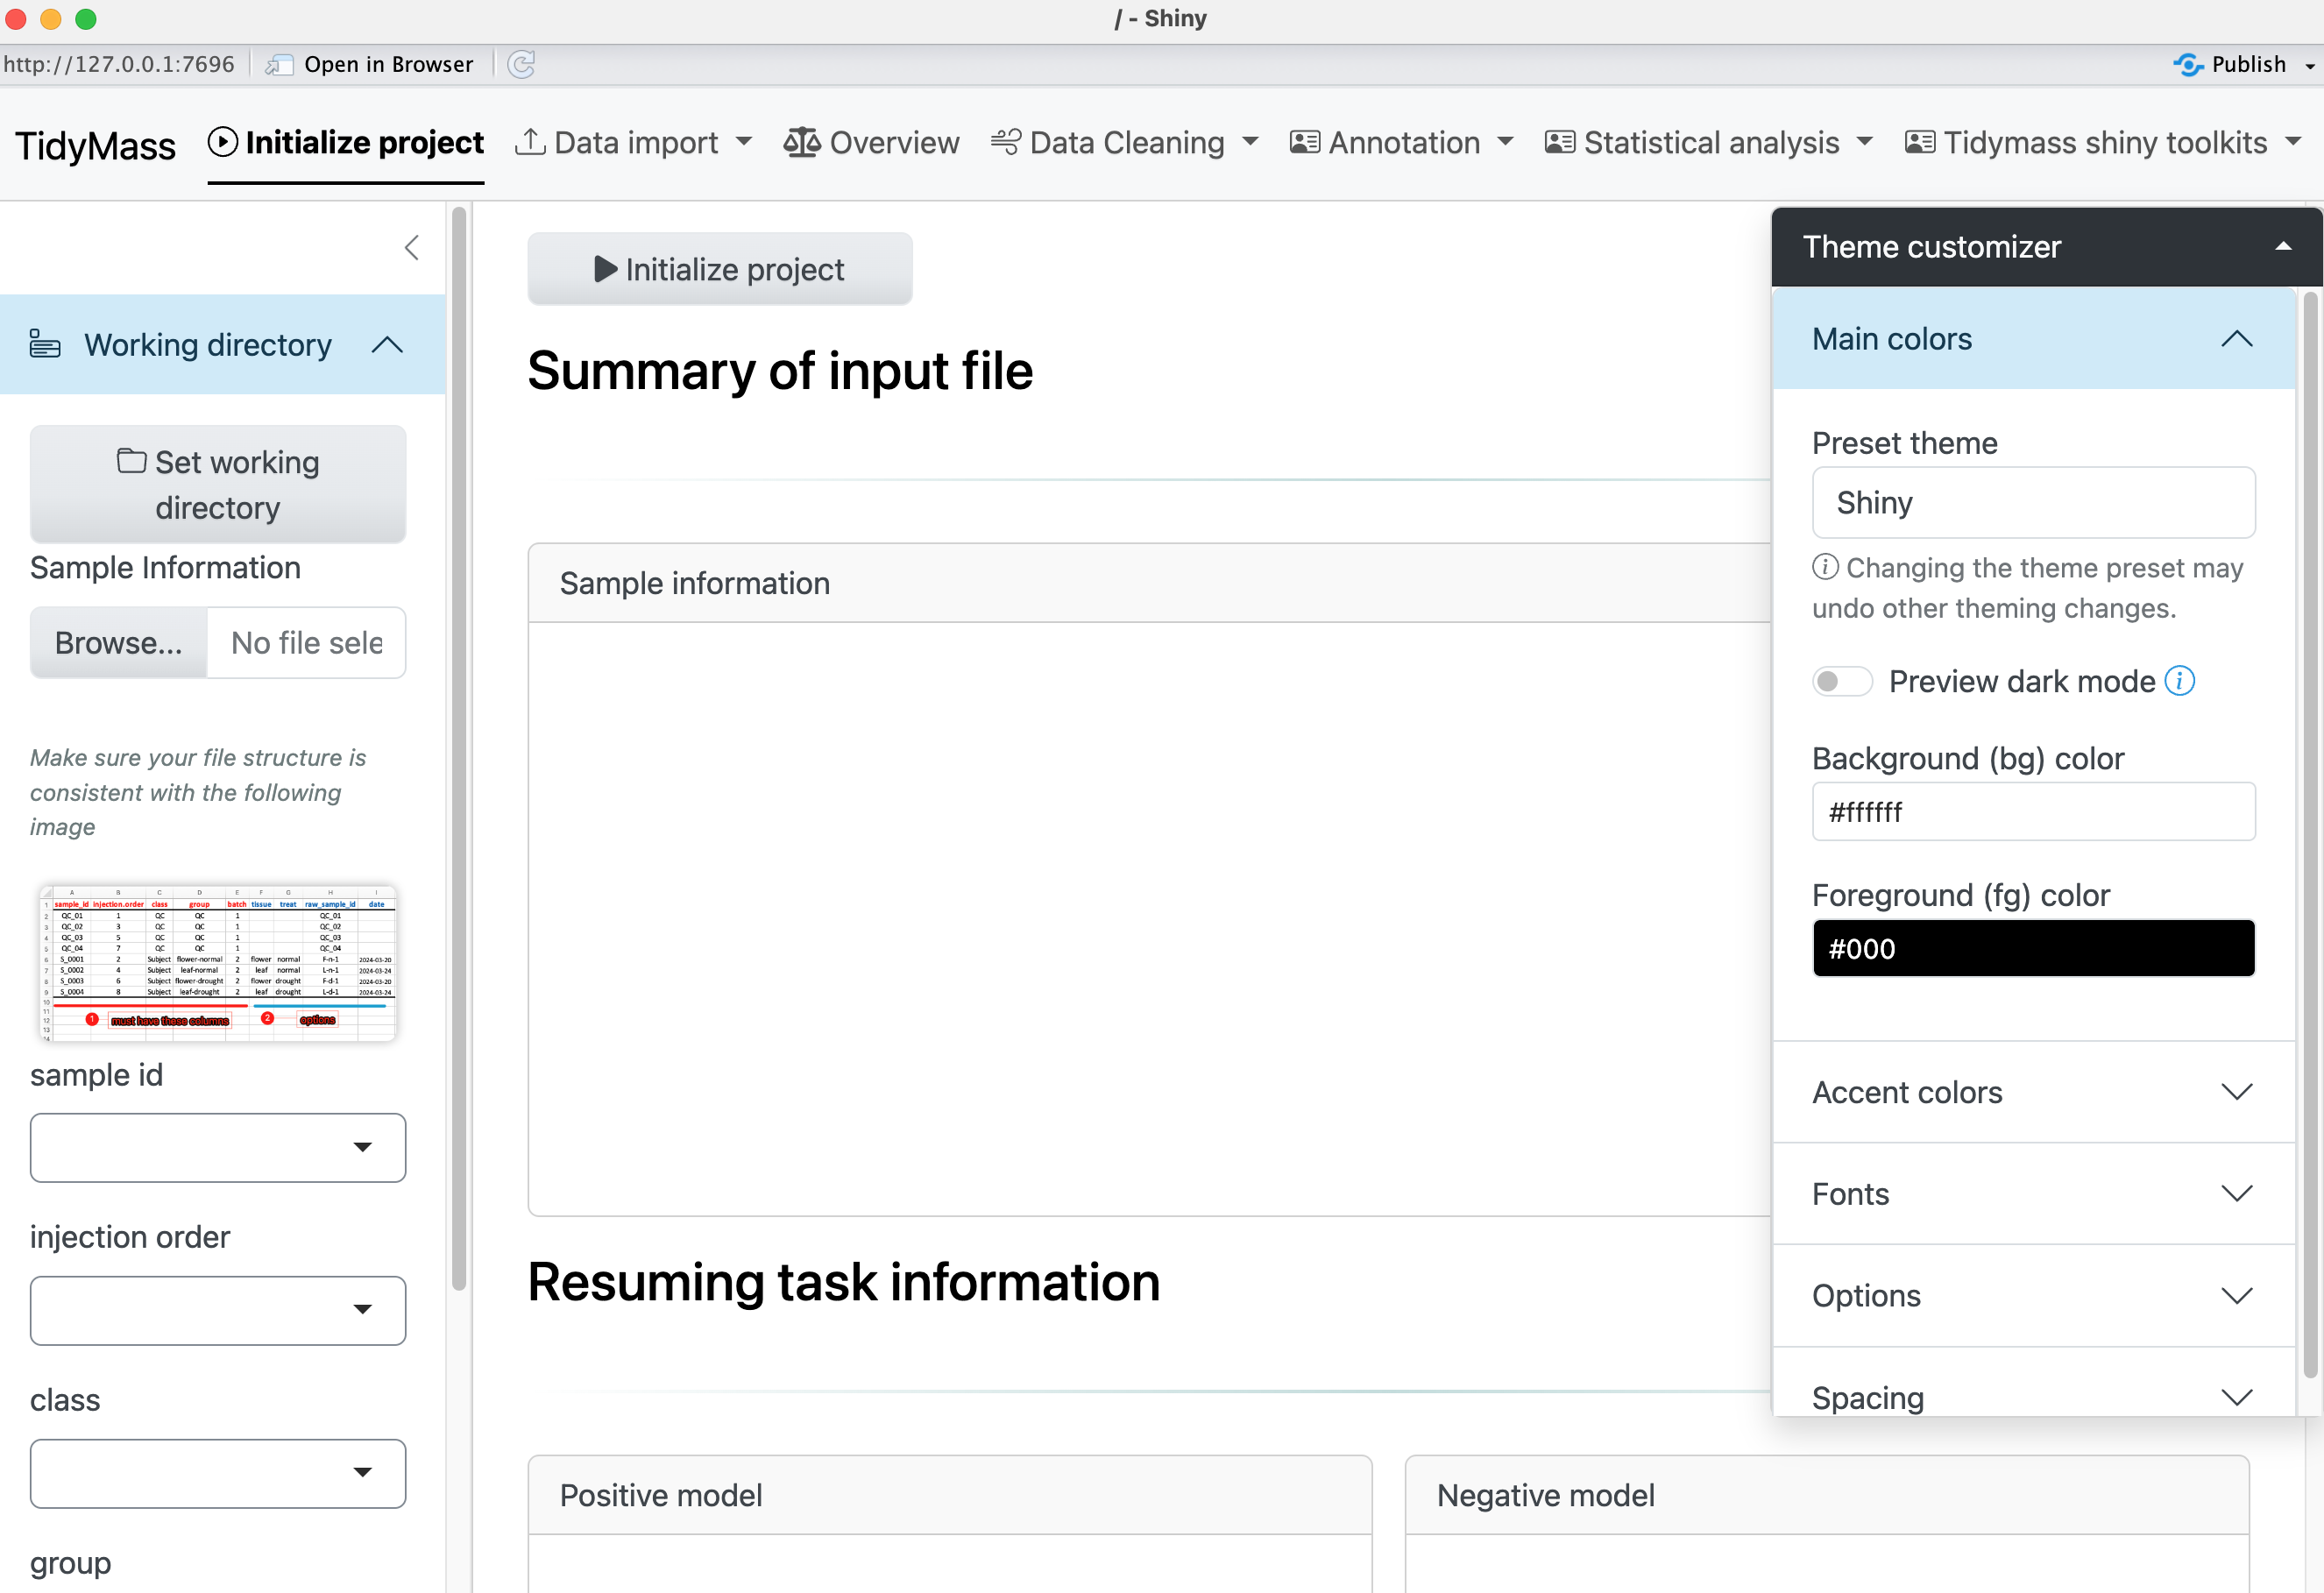
\includegraphics{figures/shinyapp.png}

To update the app to the newest version, you can run the code.

\begin{Shaded}
\begin{Highlighting}[]
\NormalTok{remotes}\SpecialCharTok{::}\FunctionTok{install\_github}\NormalTok{(}\StringTok{\textquotesingle{}tidymass/tidymass\_shiny\textquotesingle{}}\NormalTok{)}
\end{Highlighting}
\end{Shaded}

\textbf{Install with Docker}

\textbf{Install with Server}

\chapter{Upstream data processing}\label{upstream-data-processing}

To perform multiple analysis with Tidymass shinyapp, you need to upload files first, the demo data can be downloaded through \href{https://drive.google.com/file/d/10OmQjZApoqJcd163X5C67pij2yZGWHnF/view?usp=sharing}{Google Drive} or \href{https://pan.baidu.com/s/1QfwGN29dJ5mxtKmKUBo9NA?pwd=iacm}{BaiduNetdisk}.

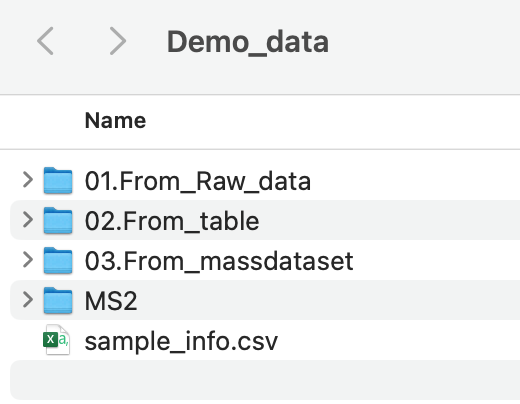
\includegraphics{figures/demo_data.png}

\section{Data format converter}\label{data-format-converter}

If your data is in raw format, you may first convert it to .mzML or .mzXML format using \href{https://proteowizard.sourceforge.io}{ProteoWizard}. Please note that ProteoWizard only support Windows OS, you may consider \href{https://massconverter.tidymass.org}{massconverter} if you don't use Windows OS.

You can refer to the following parameter settings for ProteoWizard.

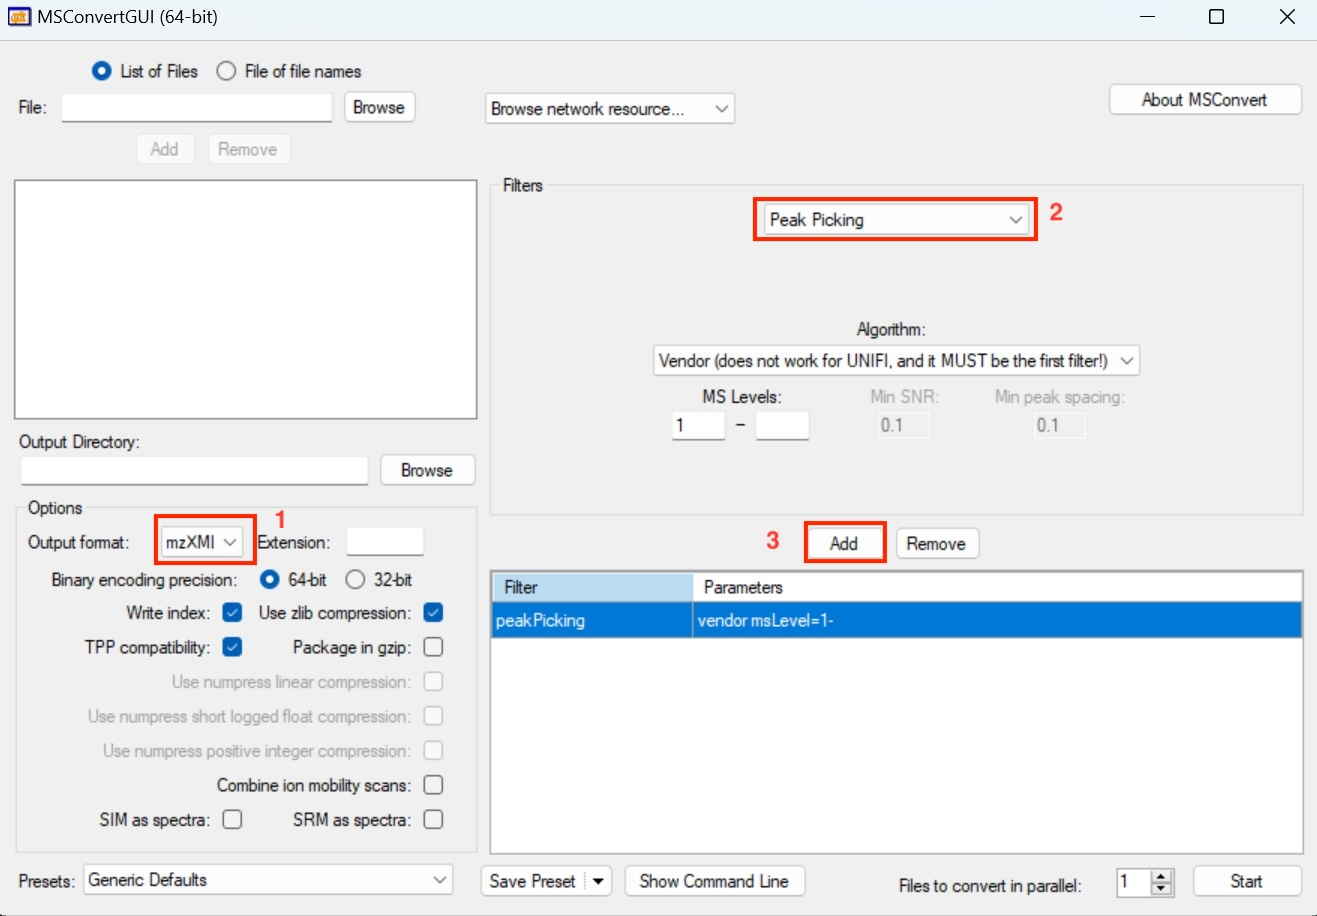
\includegraphics{figures/ProteoWizard.png}

\section{Methods to upload the files}\label{methods-to-upload-the-files}

To begin with, you need to set up the working directory and upload the required files. Here we provide three options to do that.

\textbf{Start with Ms file}:
If you have raw data in the format like .mzML or mzXML. You can click on `Start with Ms file' to upload the file.

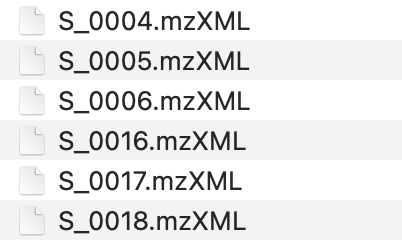
\includegraphics{figures/mzXML.png}

\textbf{Start with table file}: If your data is a post-peak metabolite expression matrix, you can click on the `Start with table file' button to upload the data. The sample table is as follows, and the first four columns must exist, with column names not to be changed.

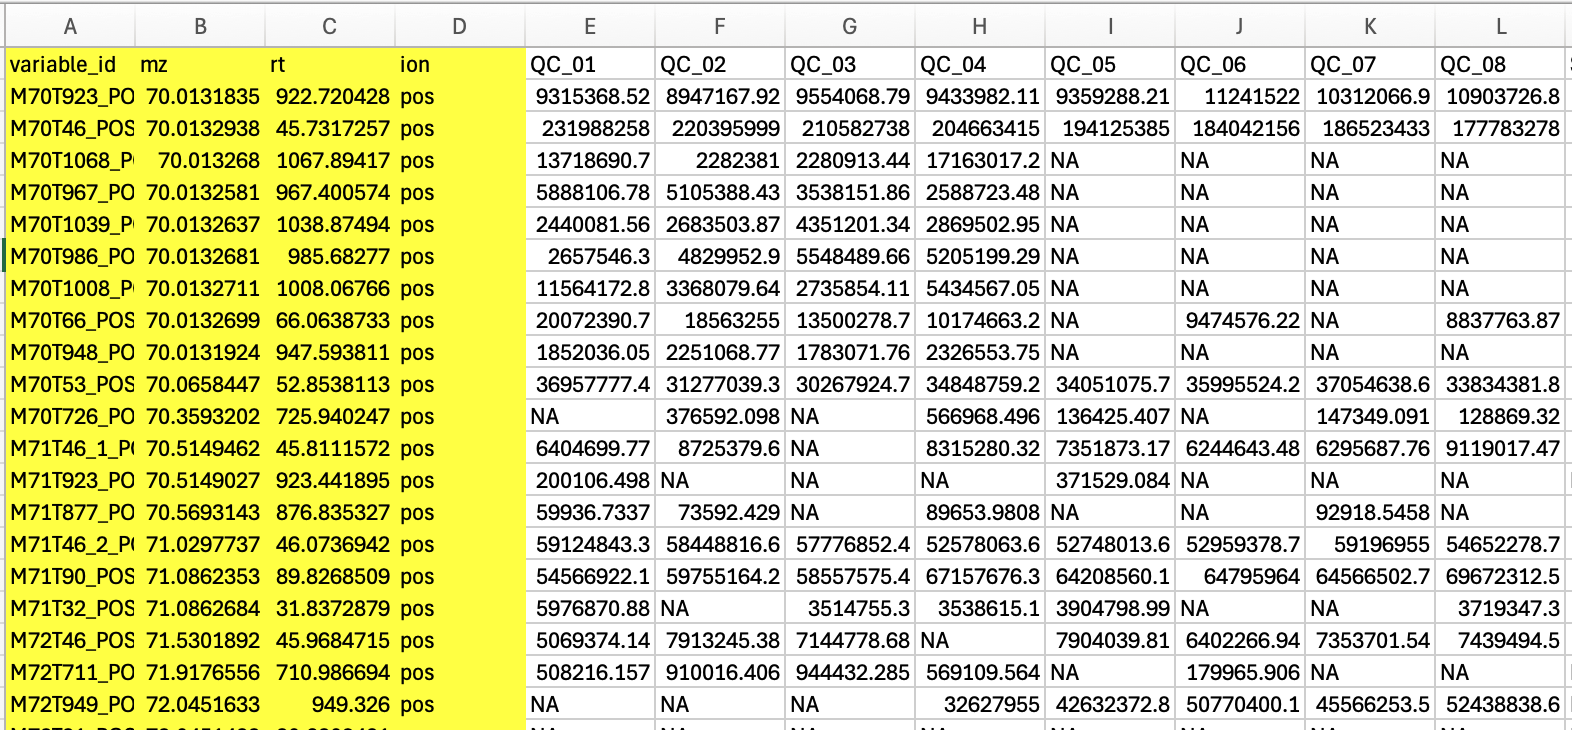
\includegraphics{figures/table_upload.png}

\textbf{Start with massdataset object}: If your data is generated by Tidymass, you can choose the `Start with massdataset object' button and directly upload them.

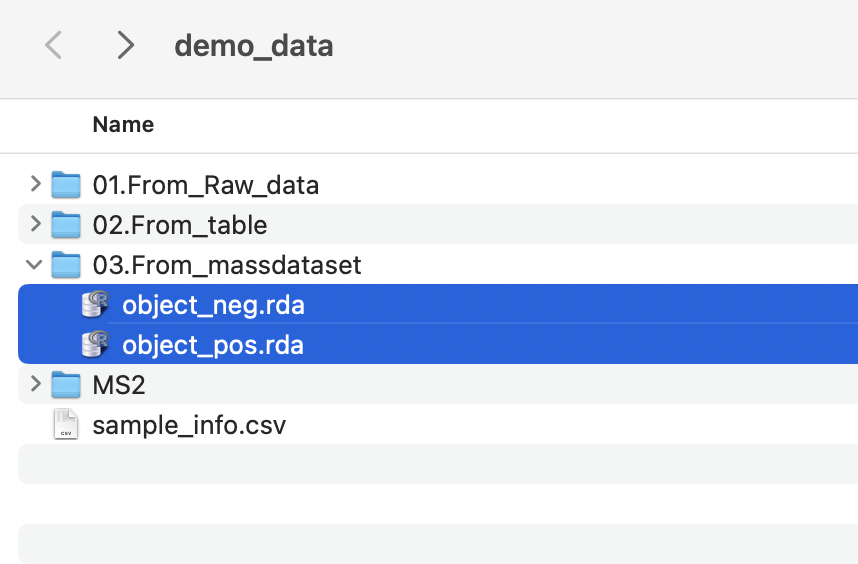
\includegraphics{figures/object_upload.png}

\section{Project initiate}\label{project-initiate}

Here are the steps you need to follow to initiate the project:

\begin{enumerate}
\def\labelenumi{\arabic{enumi}.}
\tightlist
\item
  Set working directory
\item
  Upload \texttt{sample\_info.csv} file
\item
  You may click the dropdown button and adjust the column names if there are any changes for them.
\item
  Click ``Initialize Project'' button and check the sample information.
\end{enumerate}

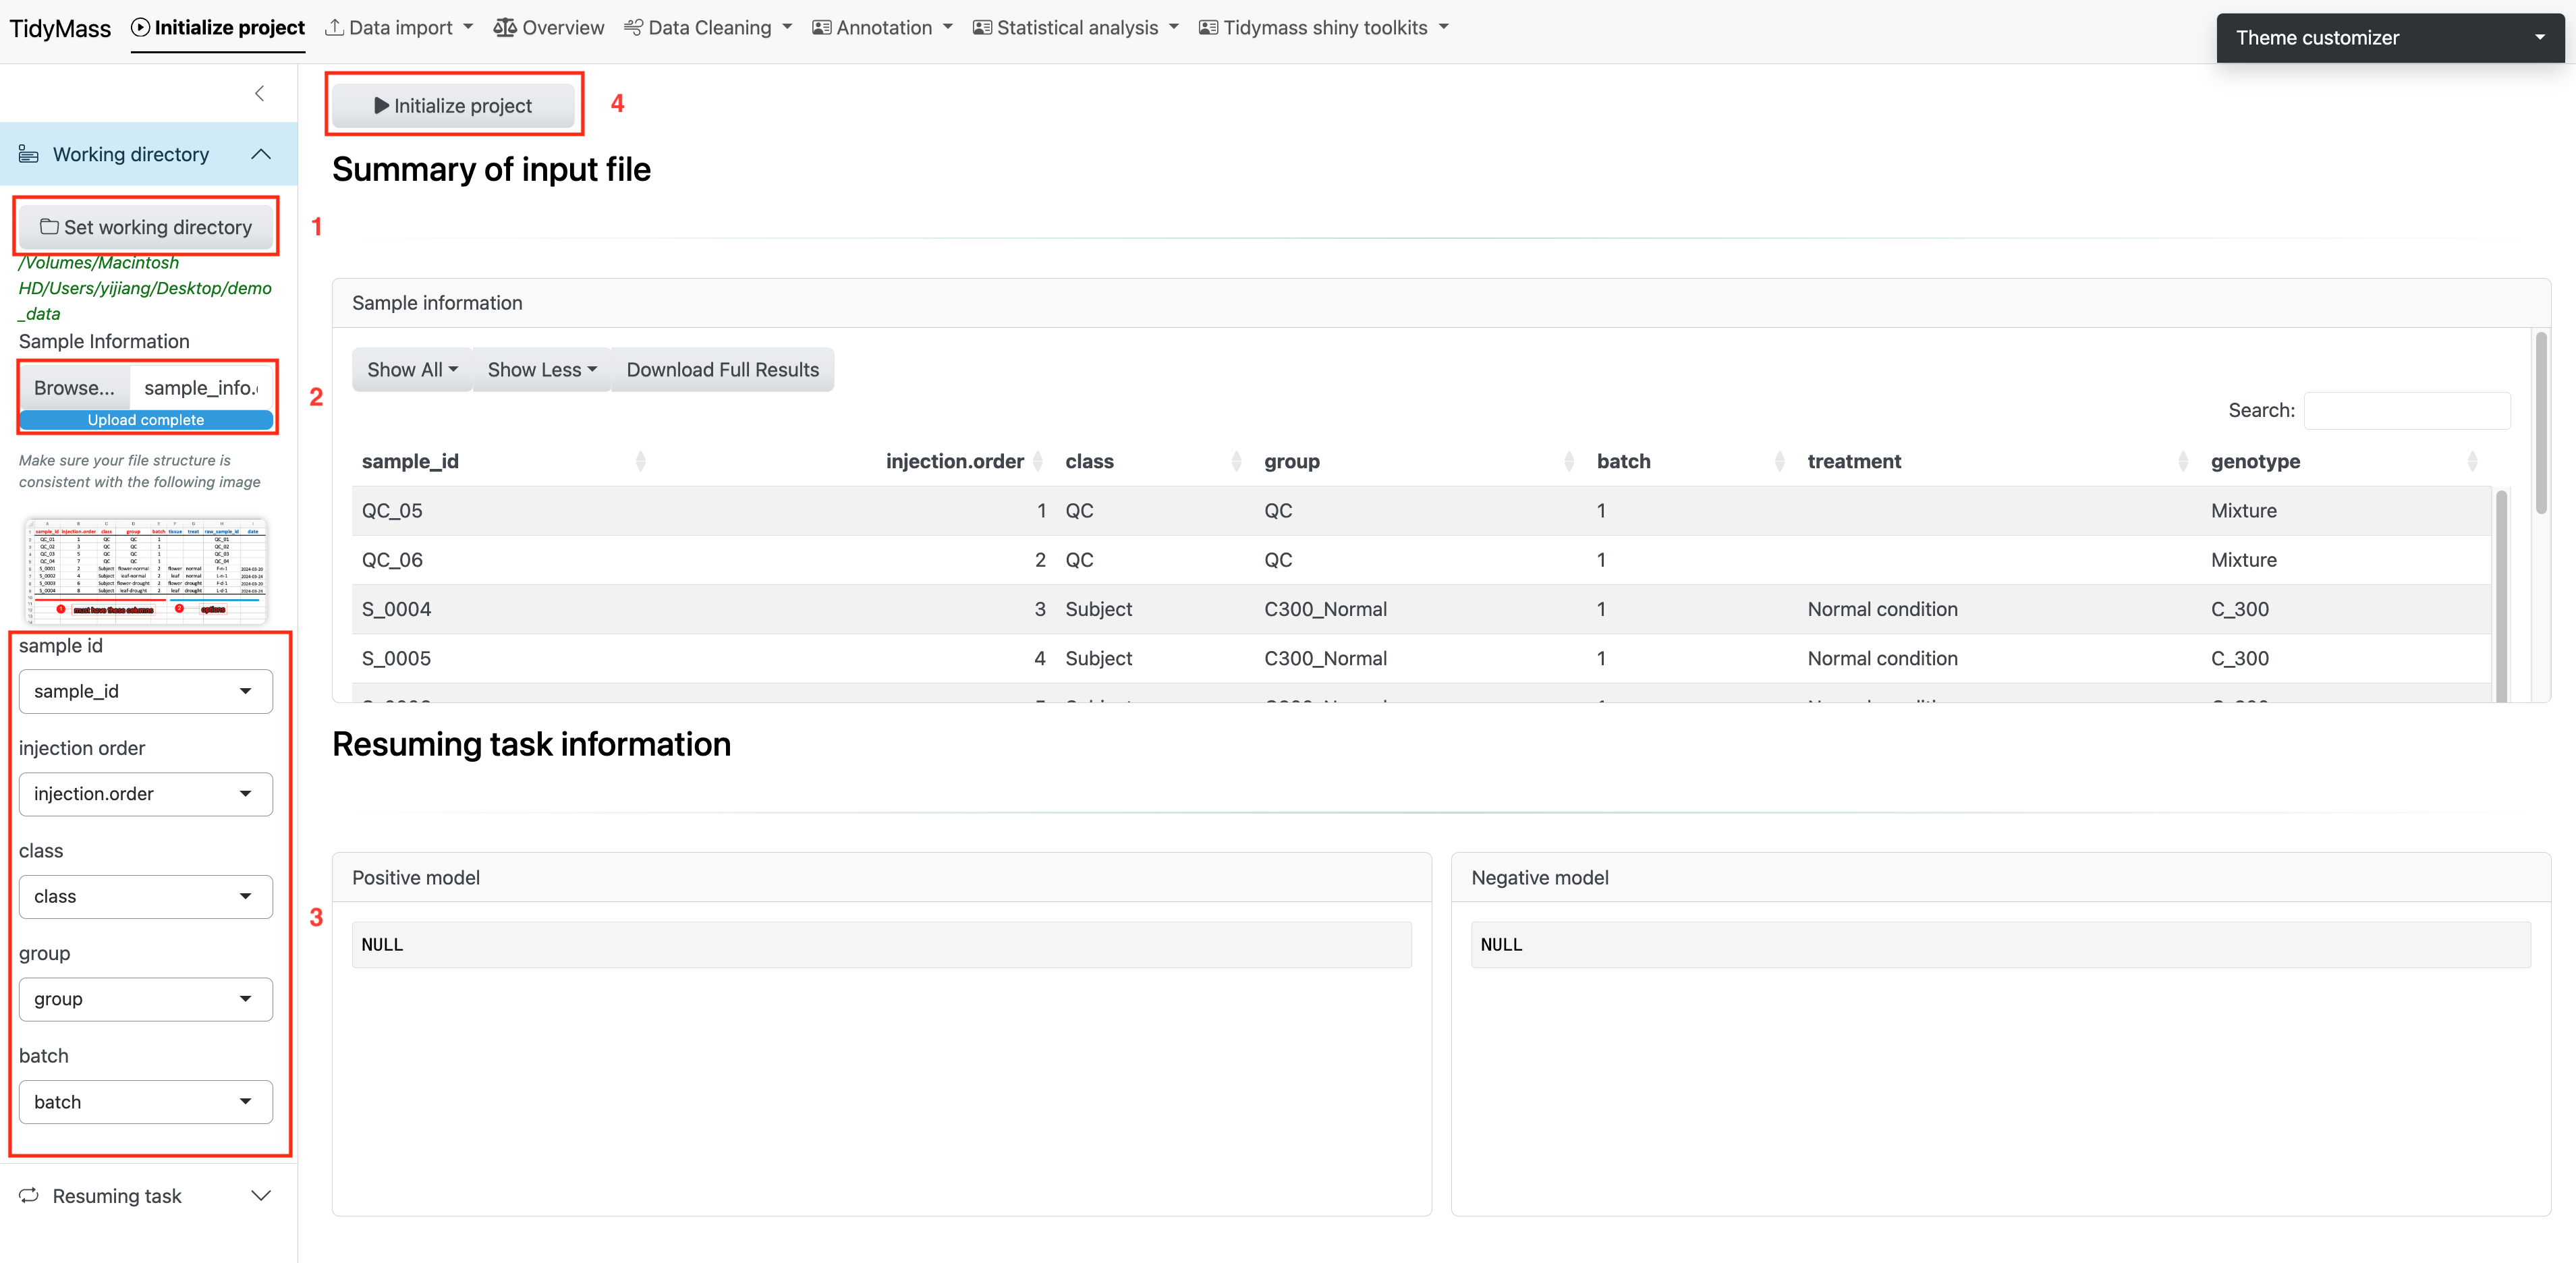
\includegraphics{figures/project_initiate.png}

\section{Data import}\label{data-import}

\textbf{Upload Ms file}

Before importing the data, please make sure the files are properly organized according to sample type, such as \texttt{QC} and \texttt{Subject}. Here is an example:

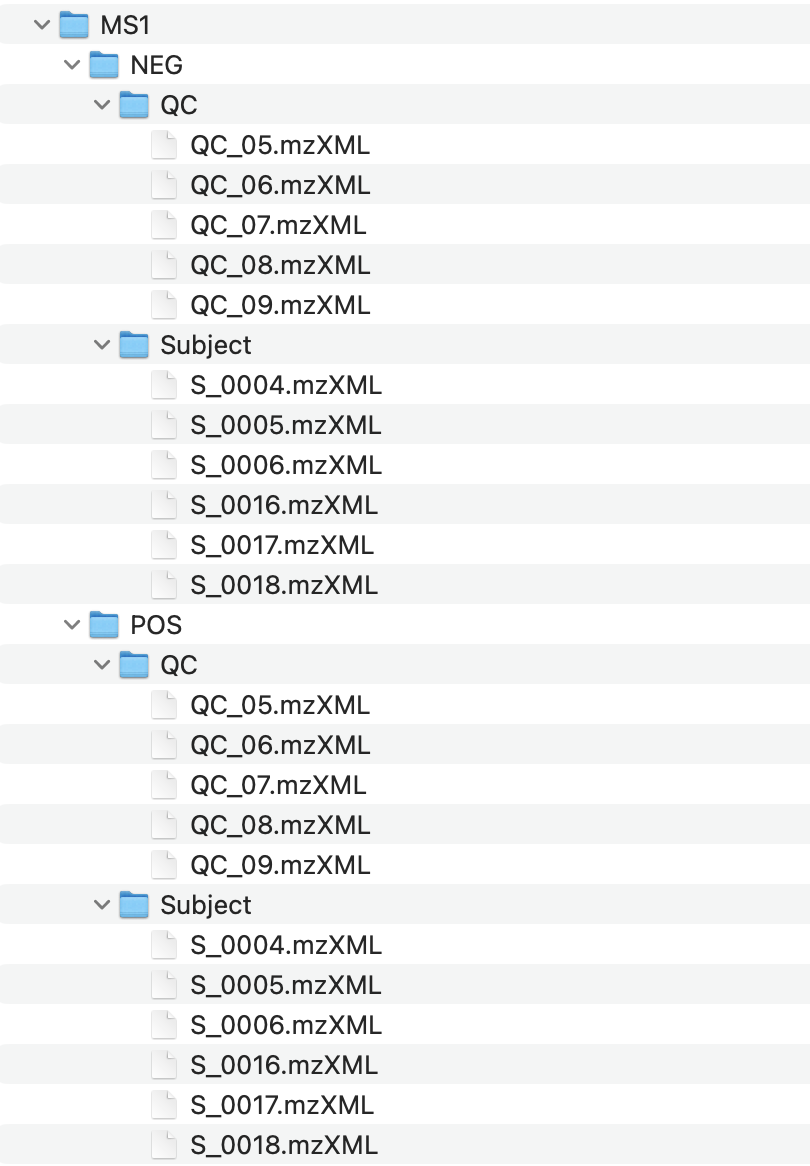
\includegraphics{figures/MS1_files.png}

Click the dropdown button \textbf{Data import} and select \textbf{Start with MS file}.

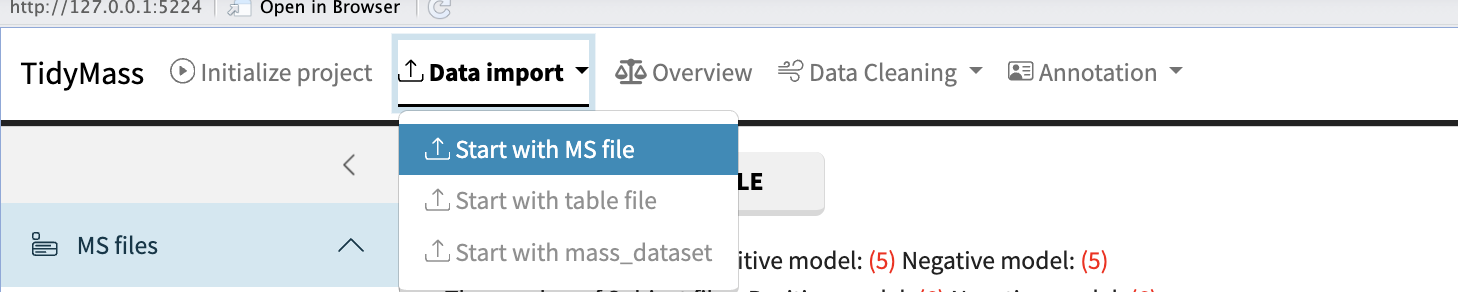
\includegraphics{figures/MS_start.png}

Then click \textbf{SELECT MS1 FOLDER} and choose the MS1 folder.

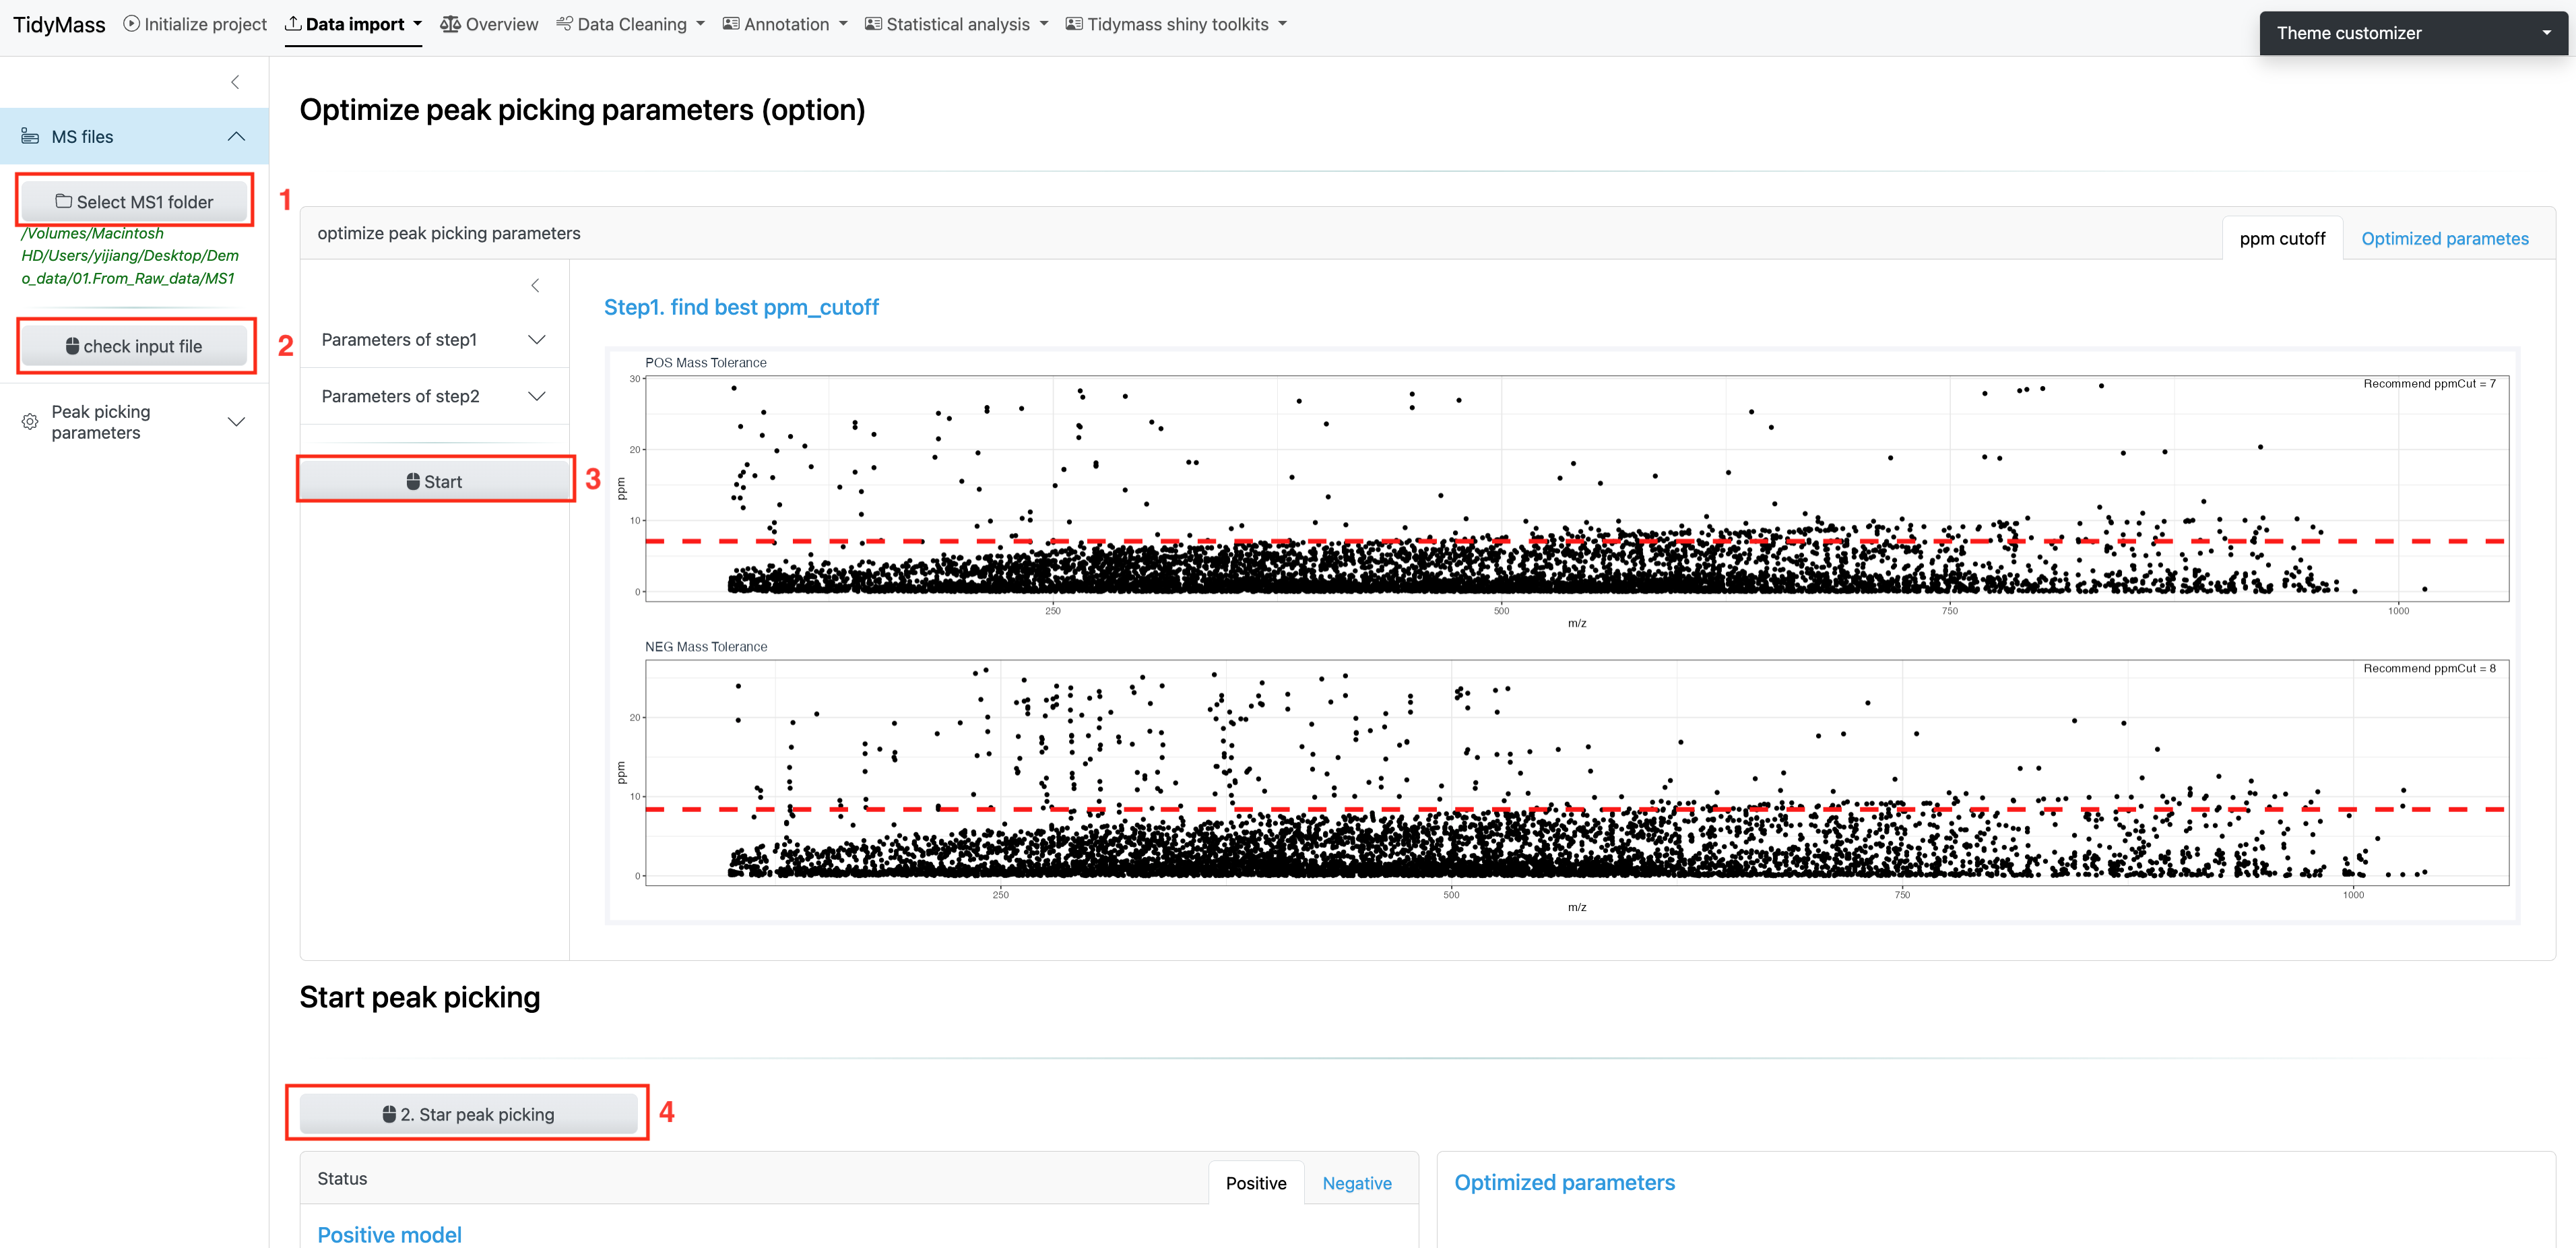
\includegraphics{figures/select_ms.png}

Next, click \textbf{CHECK INPUT FILE} and a prompt will appear if the files have been successfully uploaded.

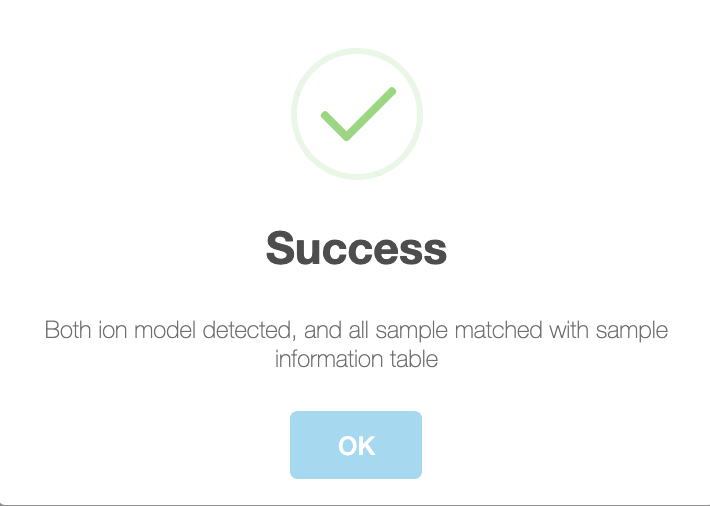
\includegraphics{figures/correct_prompt.png}

After the files are ready for analysis, you can choose to set peak picking parameters yourself. Here are some important parameters:

\begin{itemize}
\tightlist
\item
  ppm: Peak detection ppm.
\item
  peakwidth: Peak width. It is dependent on your column and LC system.
\item
  snthresh: Signal to noise threshold.
\item
  noise: Noise cutoff.
\item
  threads: The core number for performing.
\end{itemize}

For more details, please refer to \href{https://www.tidymass.org/massprocesser/articles/raw_data_processing.html}{massprocesser}.

If you want to use the recommended parameters, just click \textbf{Start} to proceed with further optimization. This will find the best ppm cutoff and run with it to perform the optimization.

Finally, click \textbf{Start peak picking} and get the results.

\textbf{Upload table file}

Click the dropdown button \textbf{Data import} and select \textbf{Start with table file}.

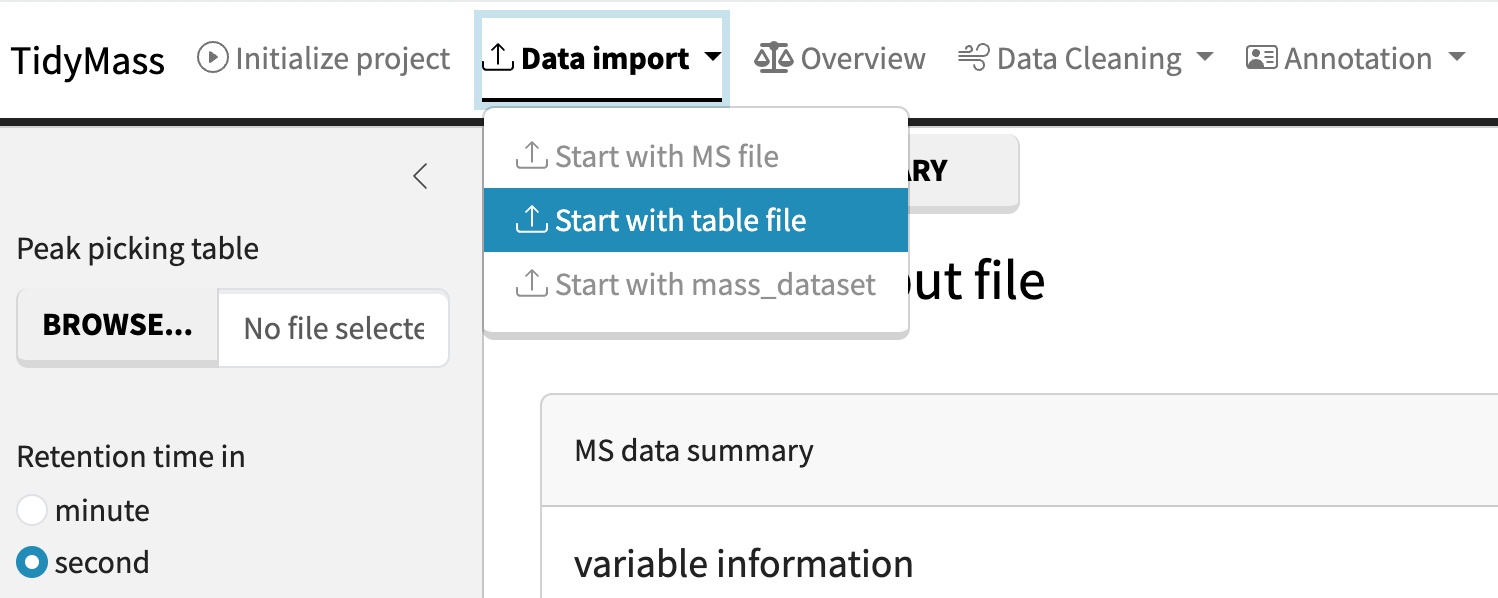
\includegraphics{figures/table_start.png}

Then click \textbf{BROWSE} and select the csv table. Next, click \textbf{INPUT FILE SUMMARY} and you will see the statistics of input file, such as \texttt{QC\ Samples}, \texttt{Subject\ Samples} and \texttt{Total\ Features}.

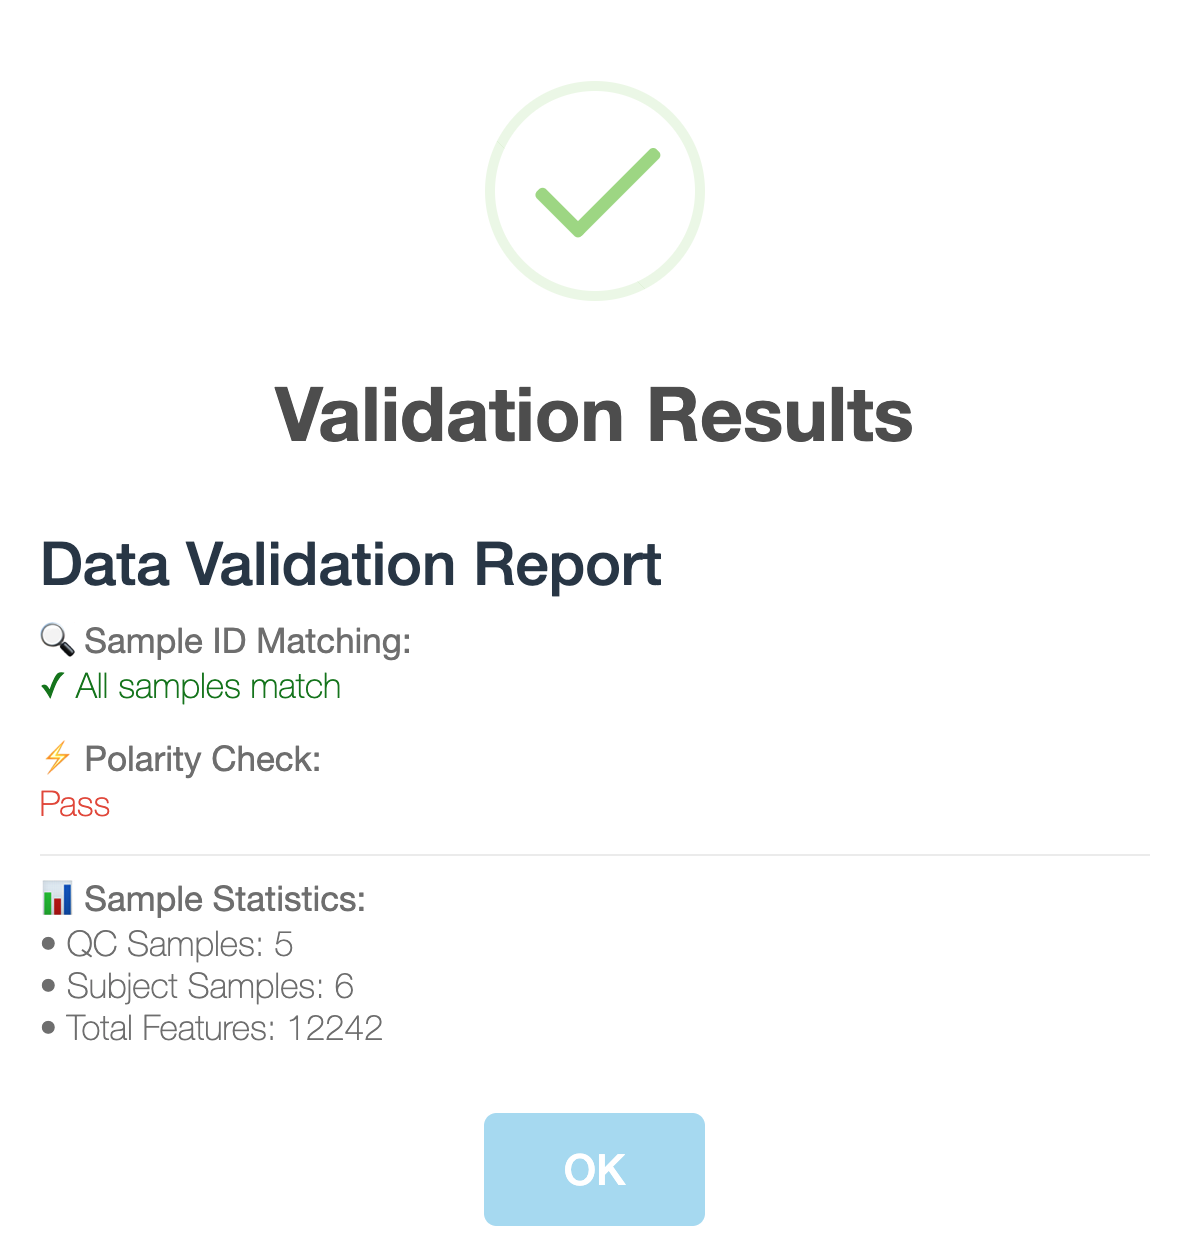
\includegraphics{figures/table_statistics.png}

If all the check have passed, click \textbf{Generate massdataset object} to obtain massdataset objects for both positive and negative modes.

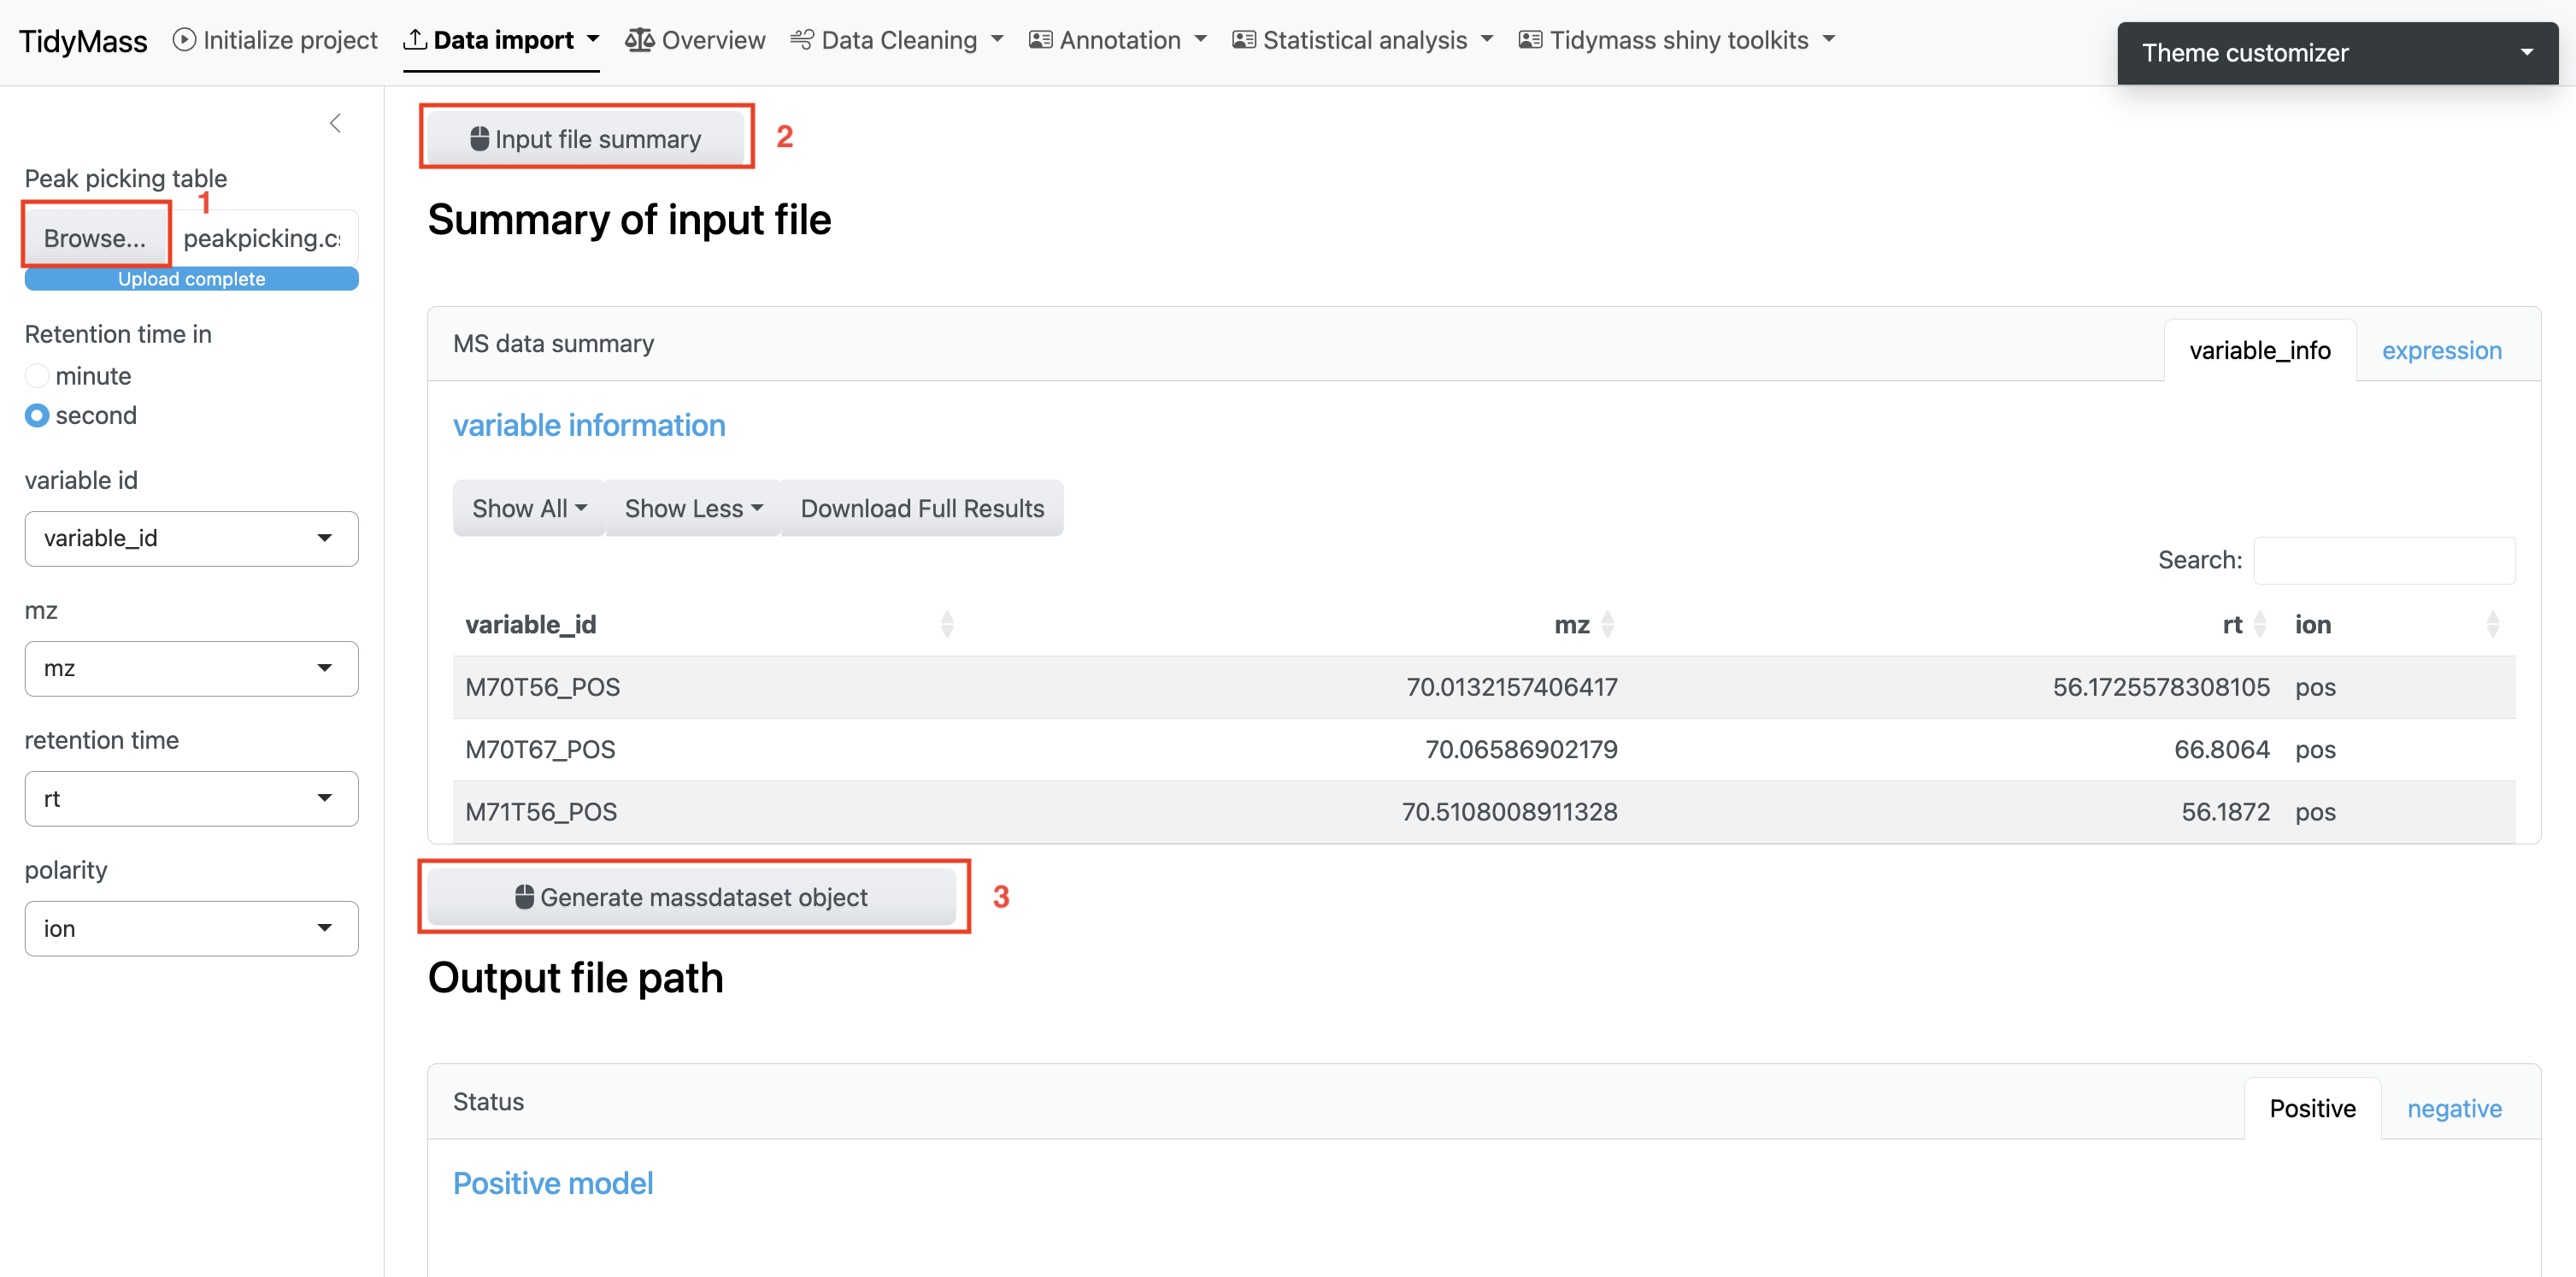
\includegraphics{figures/select_table.png}

\textbf{Upload mass\_dataset file}

If you already have massdataset objects generated by Tidymass, you can simply upload them. Upload objects for positive and negative modes separately and click \textbf{Check input}

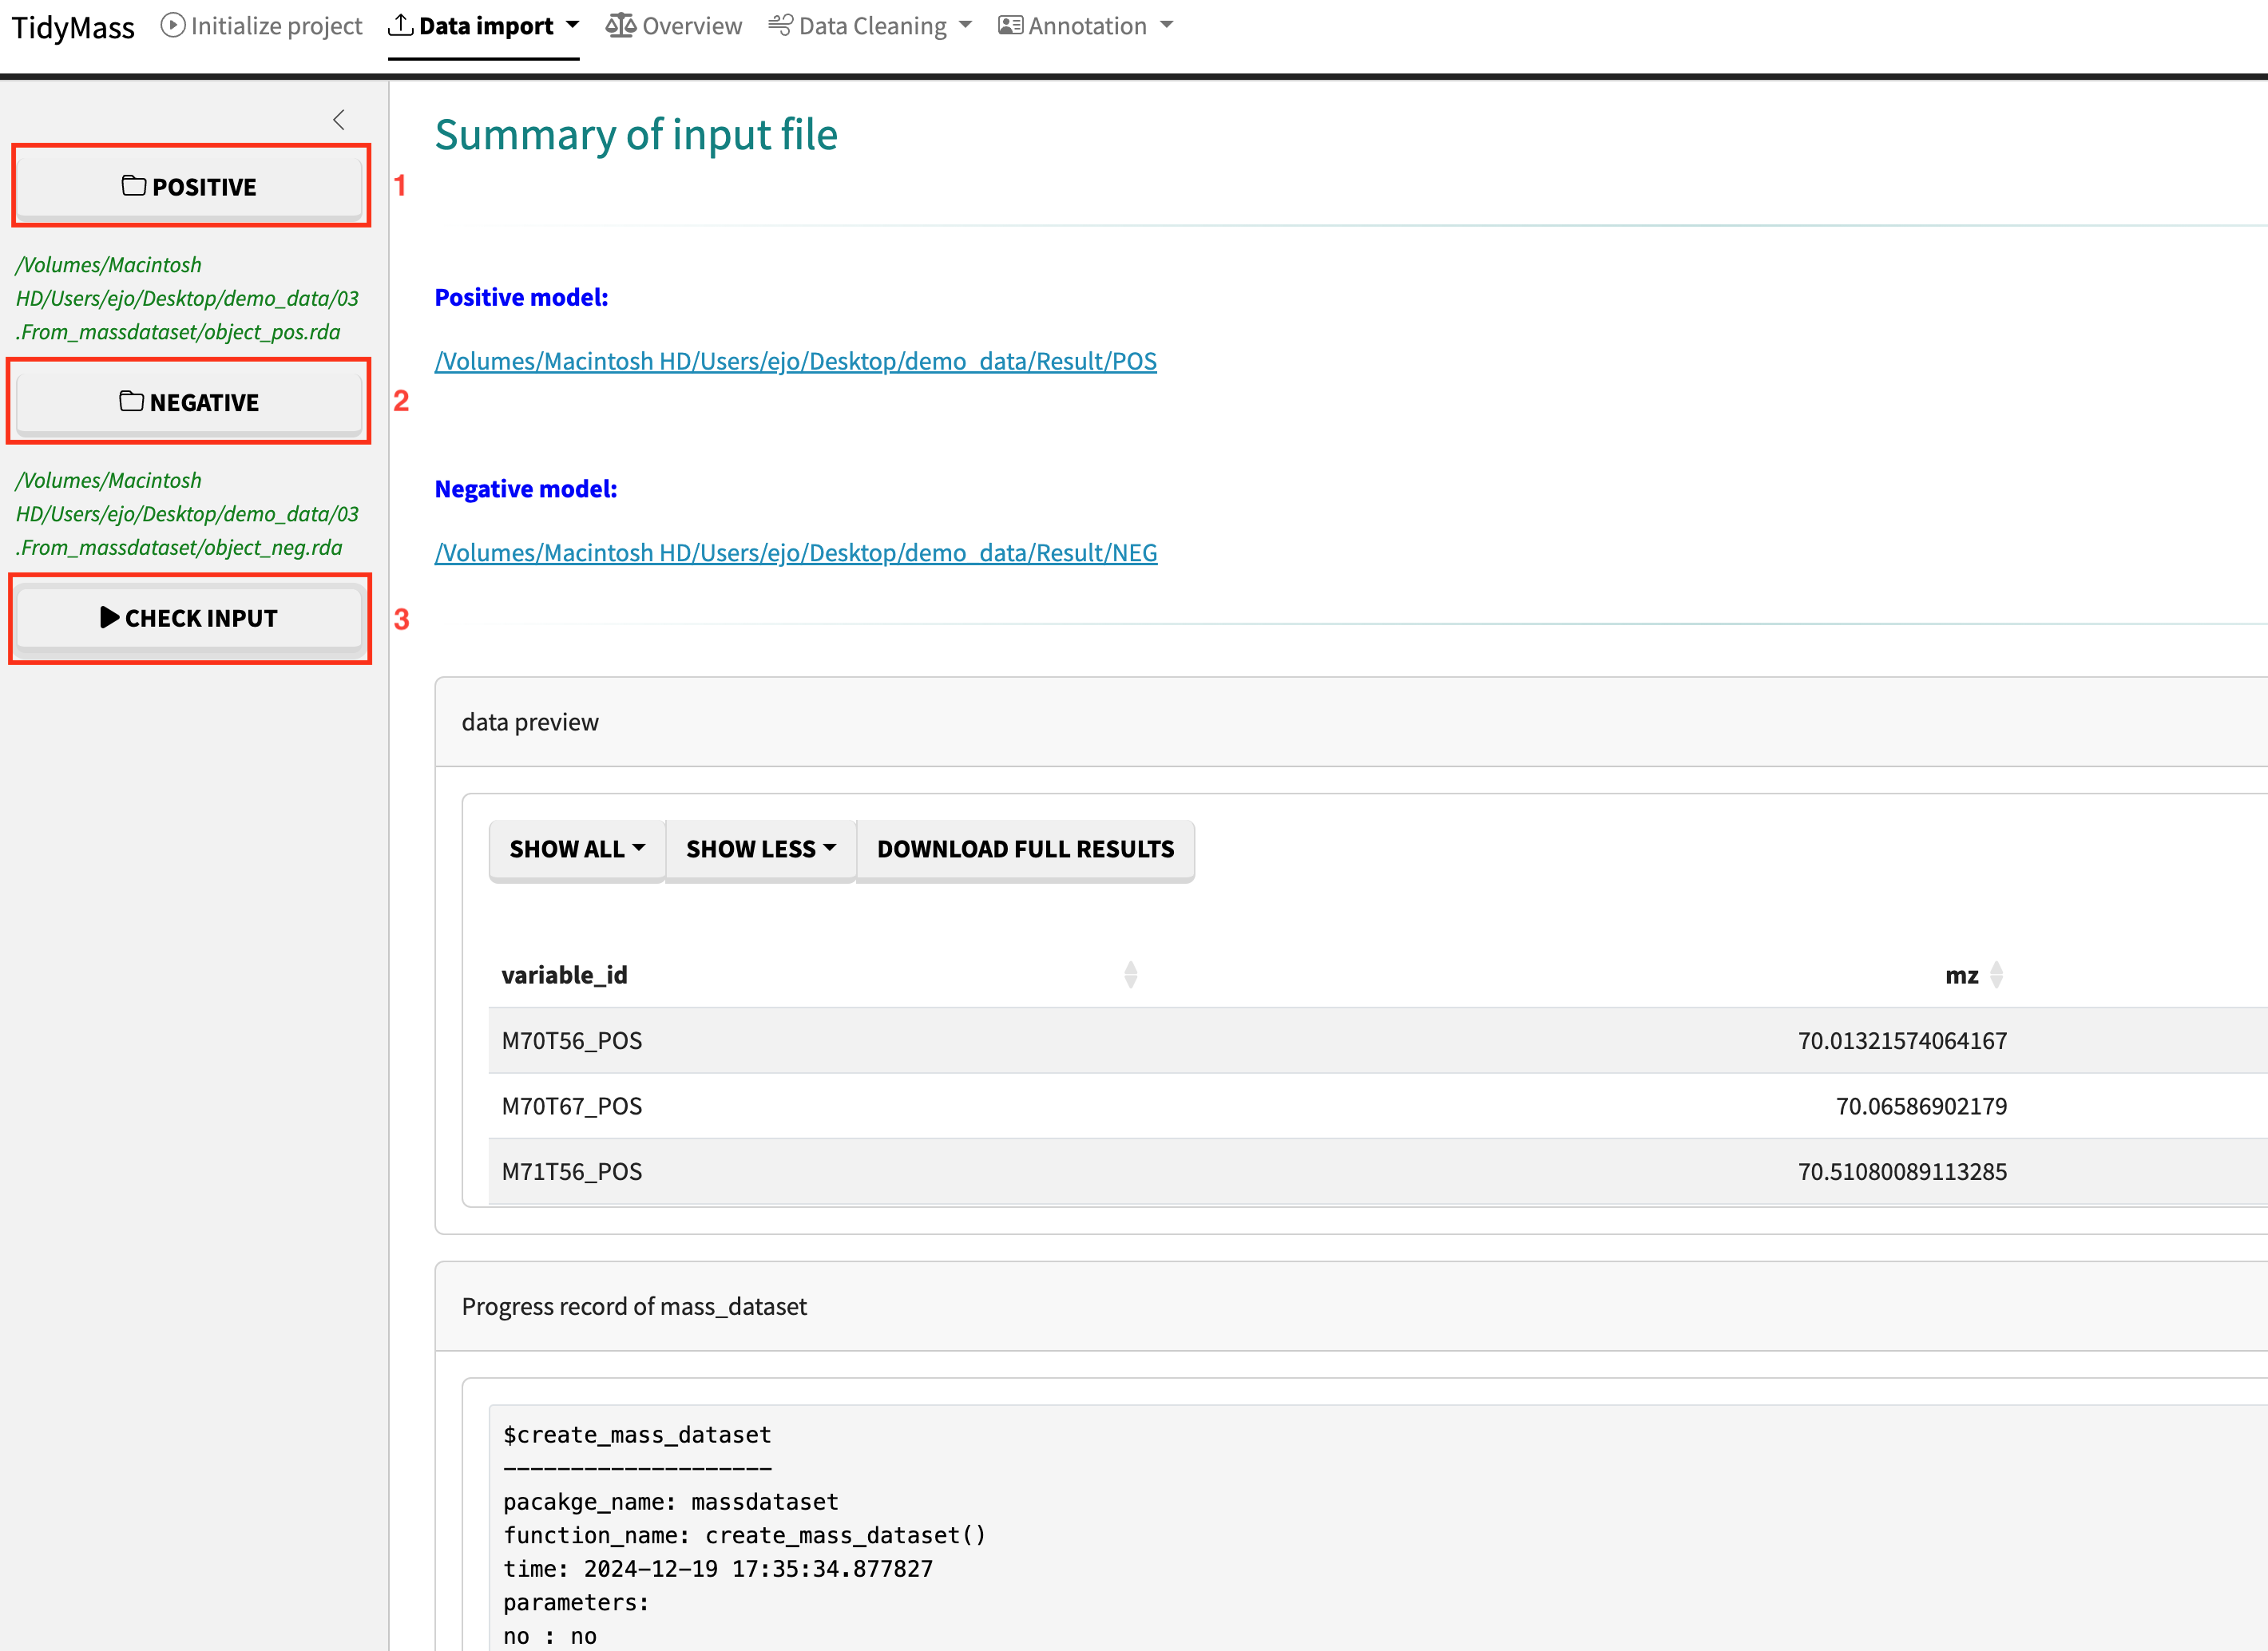
\includegraphics{figures/object_page.png}

\section{Data quaily assessment}\label{data-quaily-assessment}

To have an overall understanding and assessment of the data, you can select \textbf{Overview} and click \textbf{START} to generate multiple plots, including peak distribution, missing value summary and missing value in samples etc.

Here you can also adjust parameters and download these plots.

Multiple plots can be generated, including peak distribution plots of for two modes

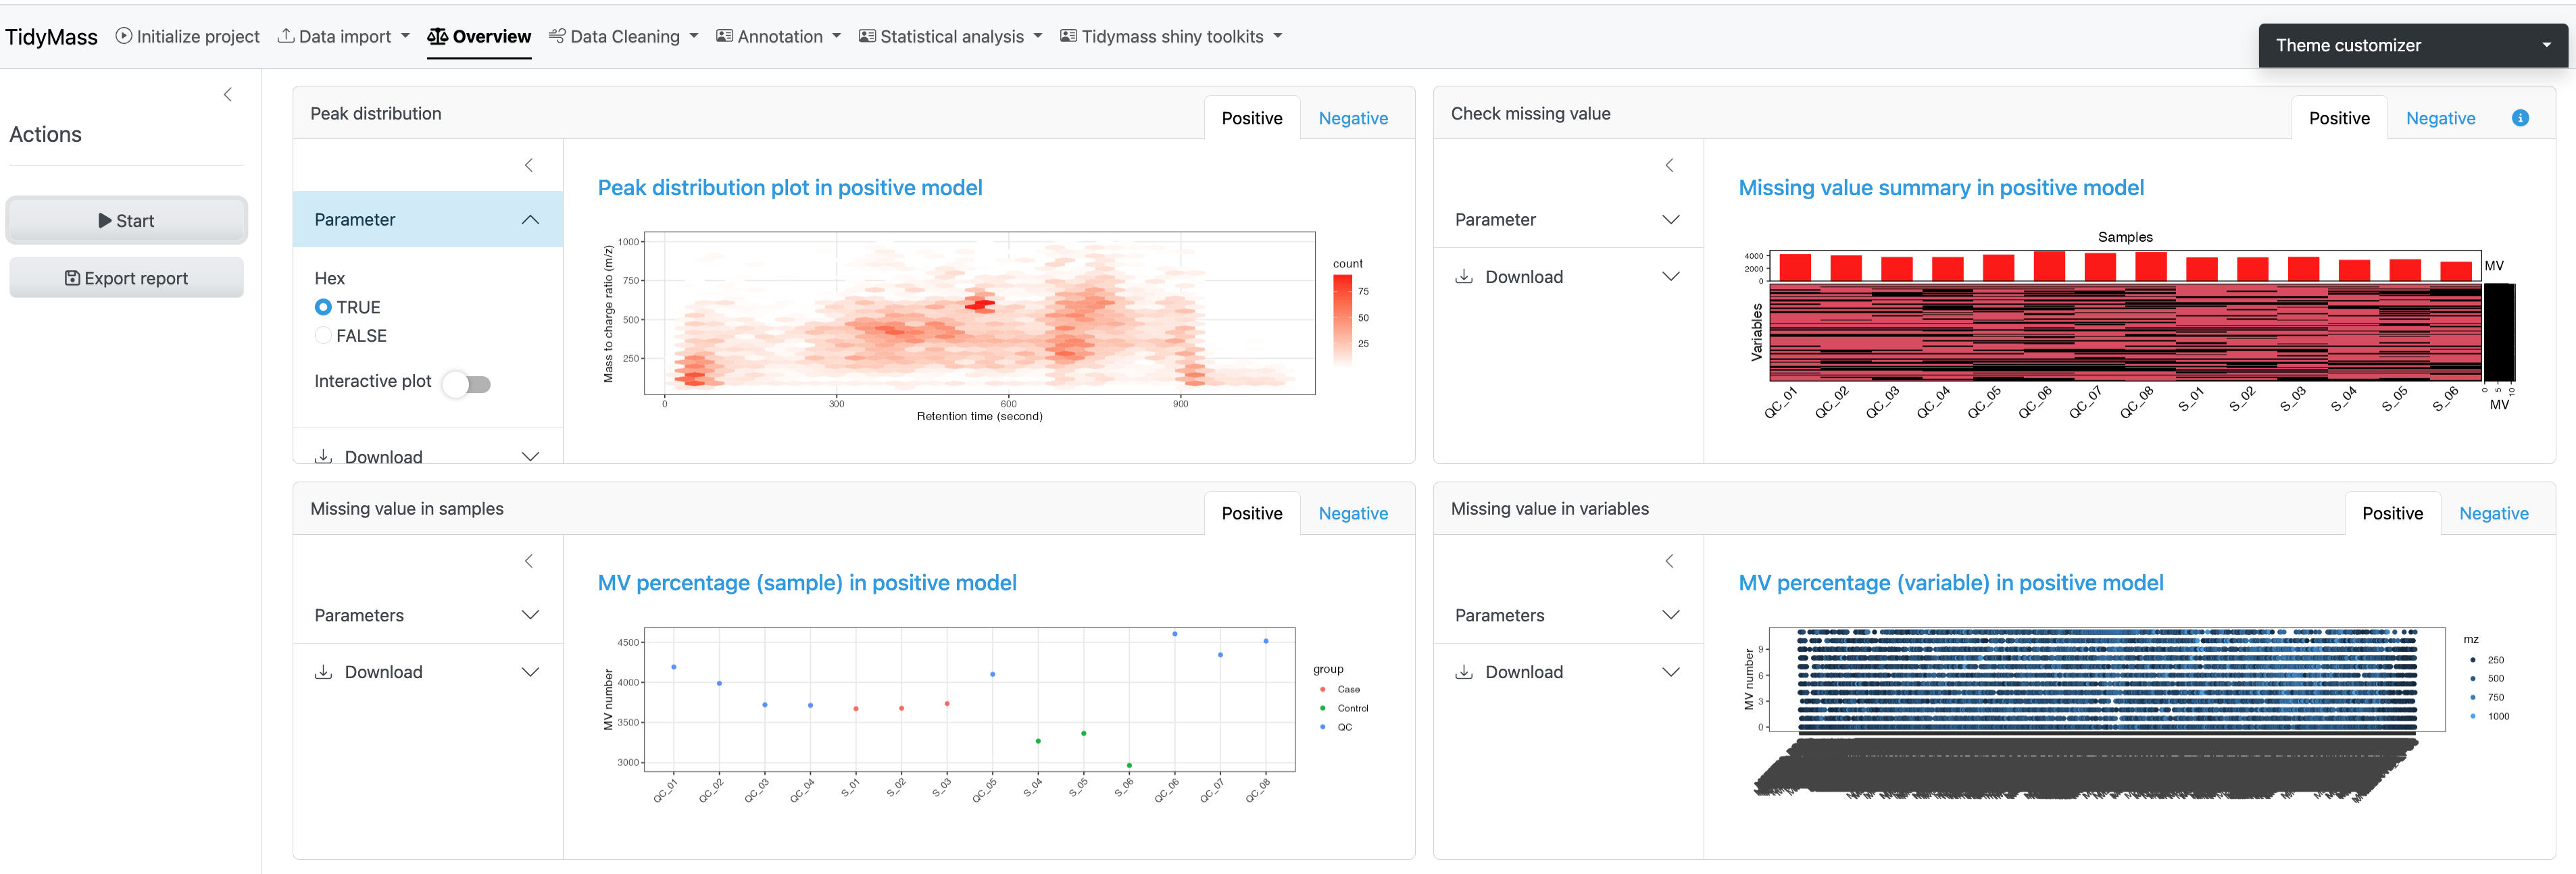
\includegraphics{figures/Overview1.png}

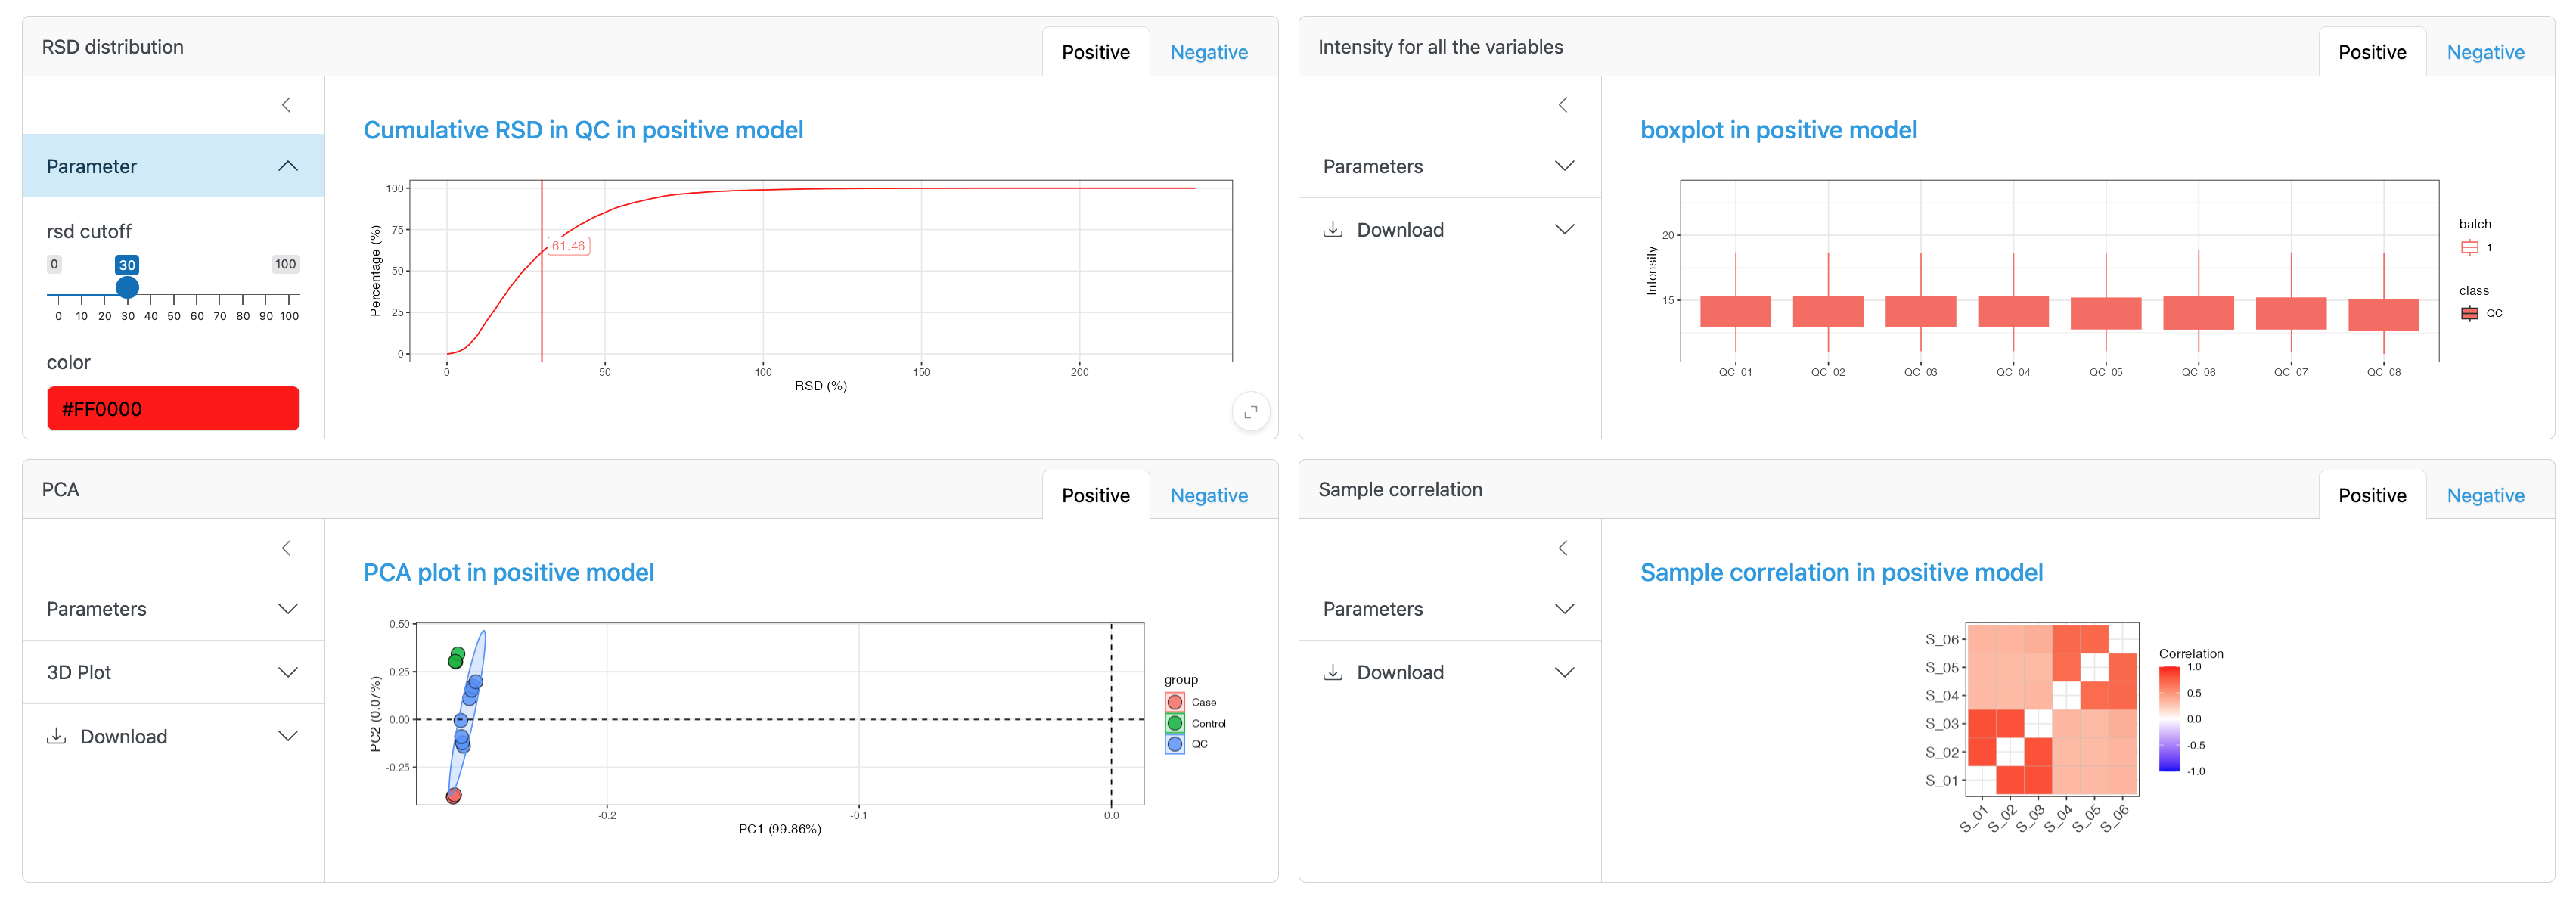
\includegraphics{figures/Overview2.png}

\section{Data cleaning}\label{data-cleaning}

Before metabolite annotation, it's necessary to perform \textbf{data cleaning} as various bias may exist in sample preparation and data acquisition. It can be divided into different steps such as noisy feature removal and outlier samples removal. For more details, please refer to \href{https://masscleaner.tidymass.org/}{masscleaner}.

\textbf{Remove noisy metabolic features}

The first step is removing noisy metabolic features. Here we choose to remove variables who have MV in more than 20\% QC samples and in at lest 50\% samples in control group or case group, so the \textbf{MV cutoff of QC samples (\%)} has been set as 20 and \textbf{MV cutoff (\%)} has been set as 50.

Click \textbf{Start} to remove these noisy metabolites.

Next, you can visualize the MV percentage of samples for \texttt{QC\ group}, \texttt{Subject\ group} or both of them by click \textbf{Show plot}.

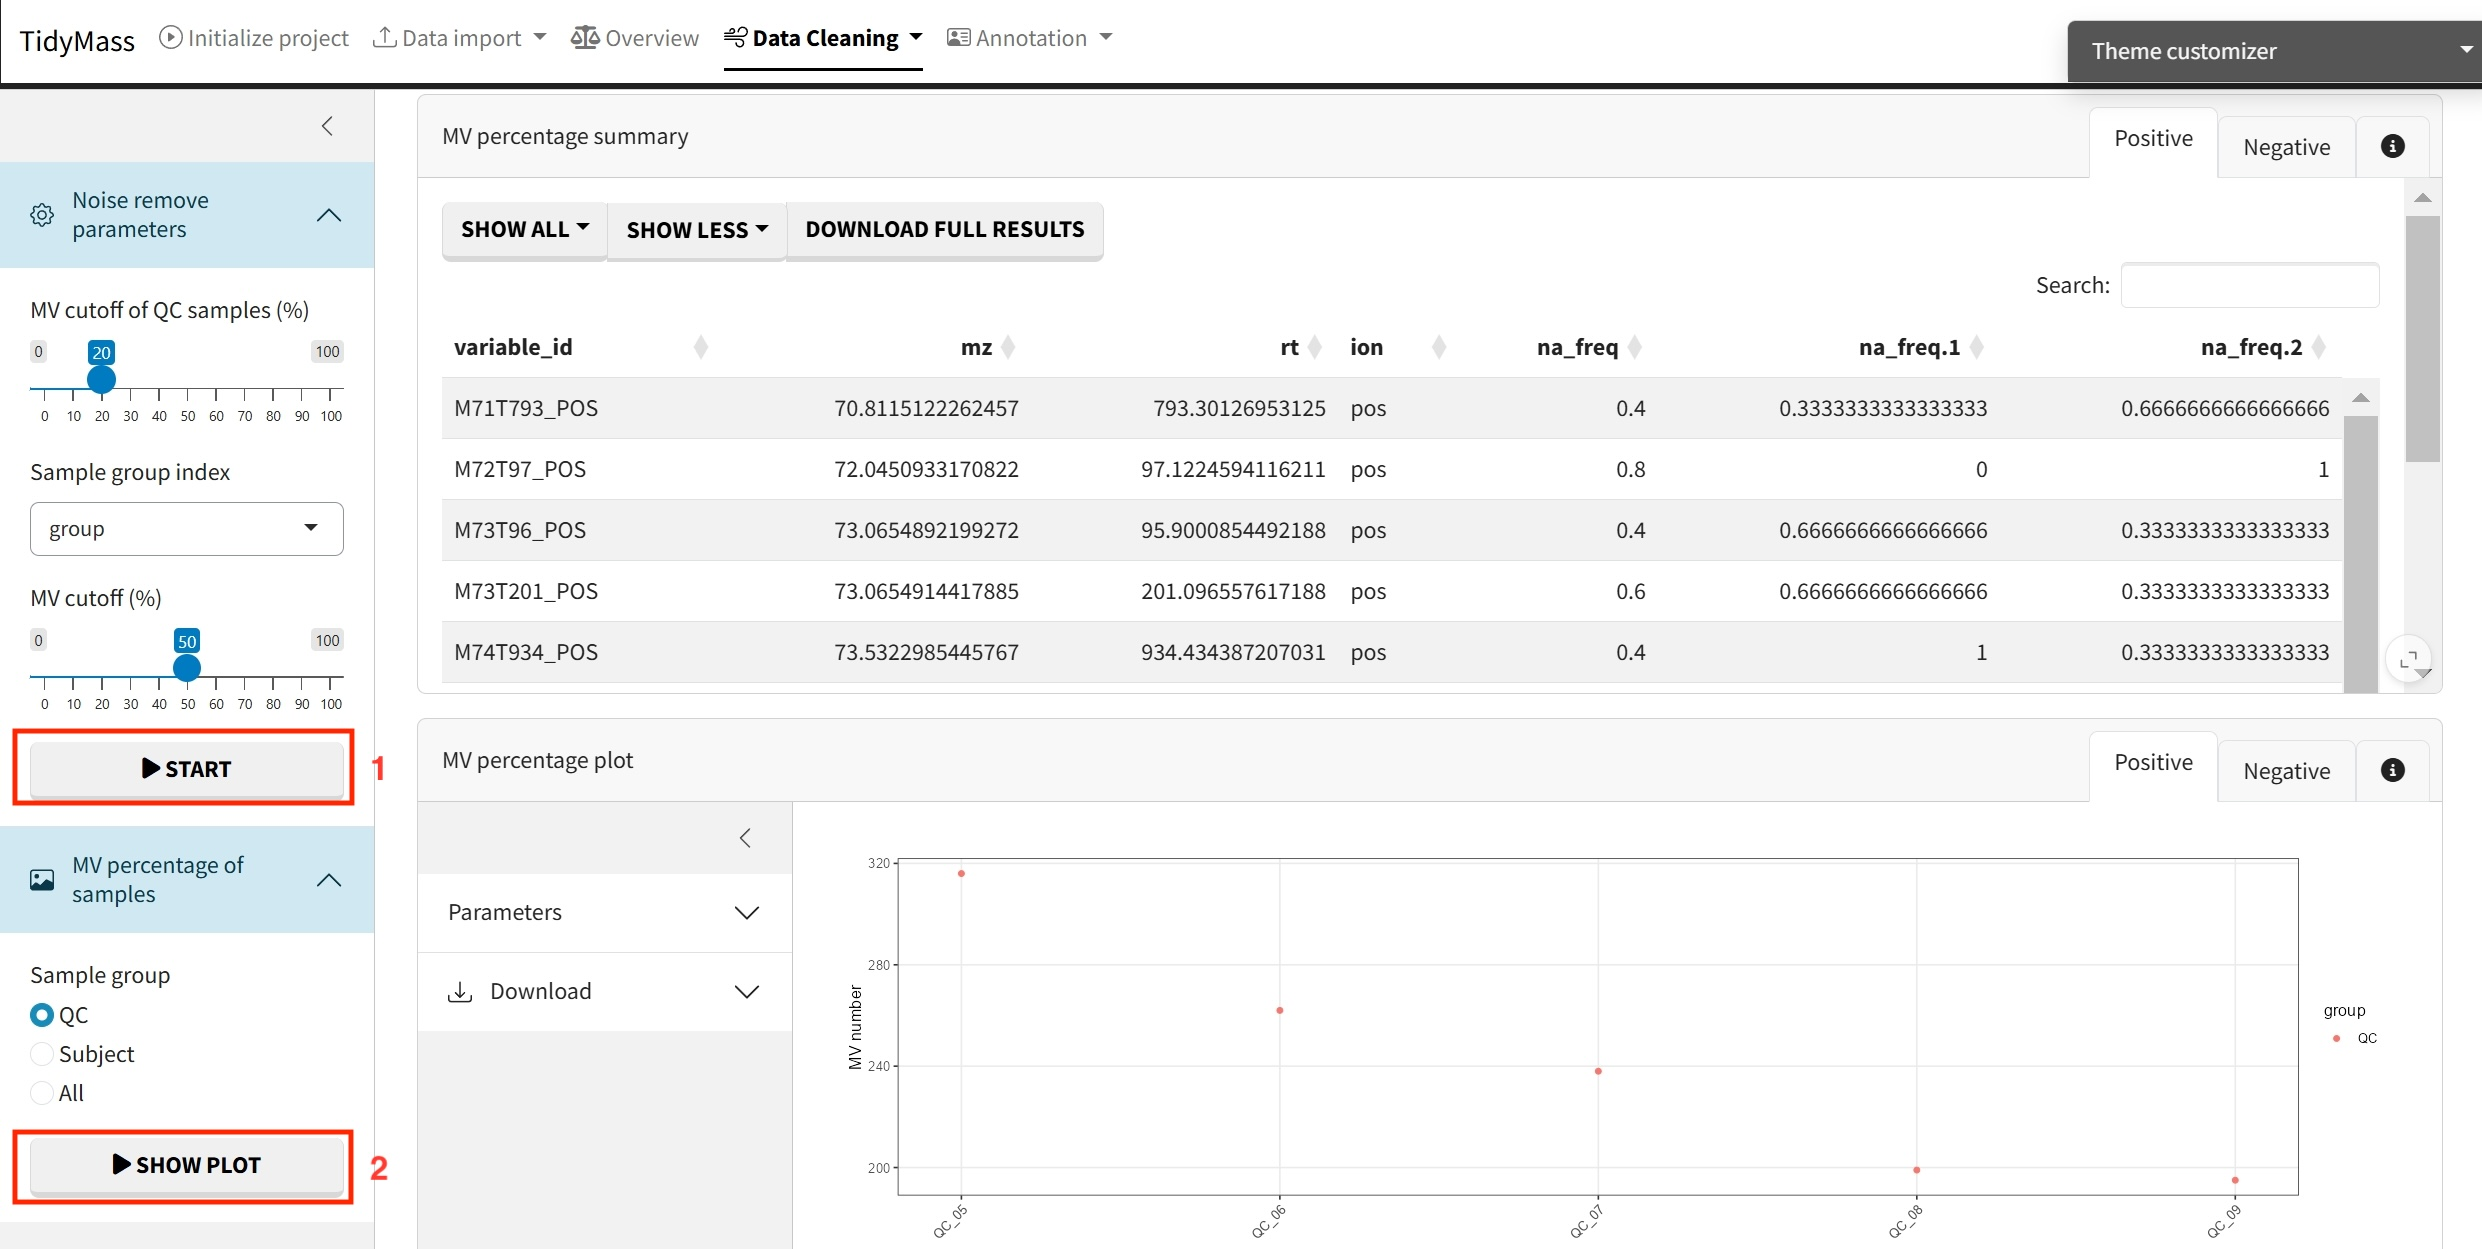
\includegraphics{figures/noisy_metabolites.png}

\textbf{Filter outlier samples}

When analyzing large cohorts, outlier samples can be a serious problem. In this step, we will filter these outlier samples.

Before filtering outlier samples, you can click \textbf{Start} above to show the plot for Missing value in samples and PCA plot.

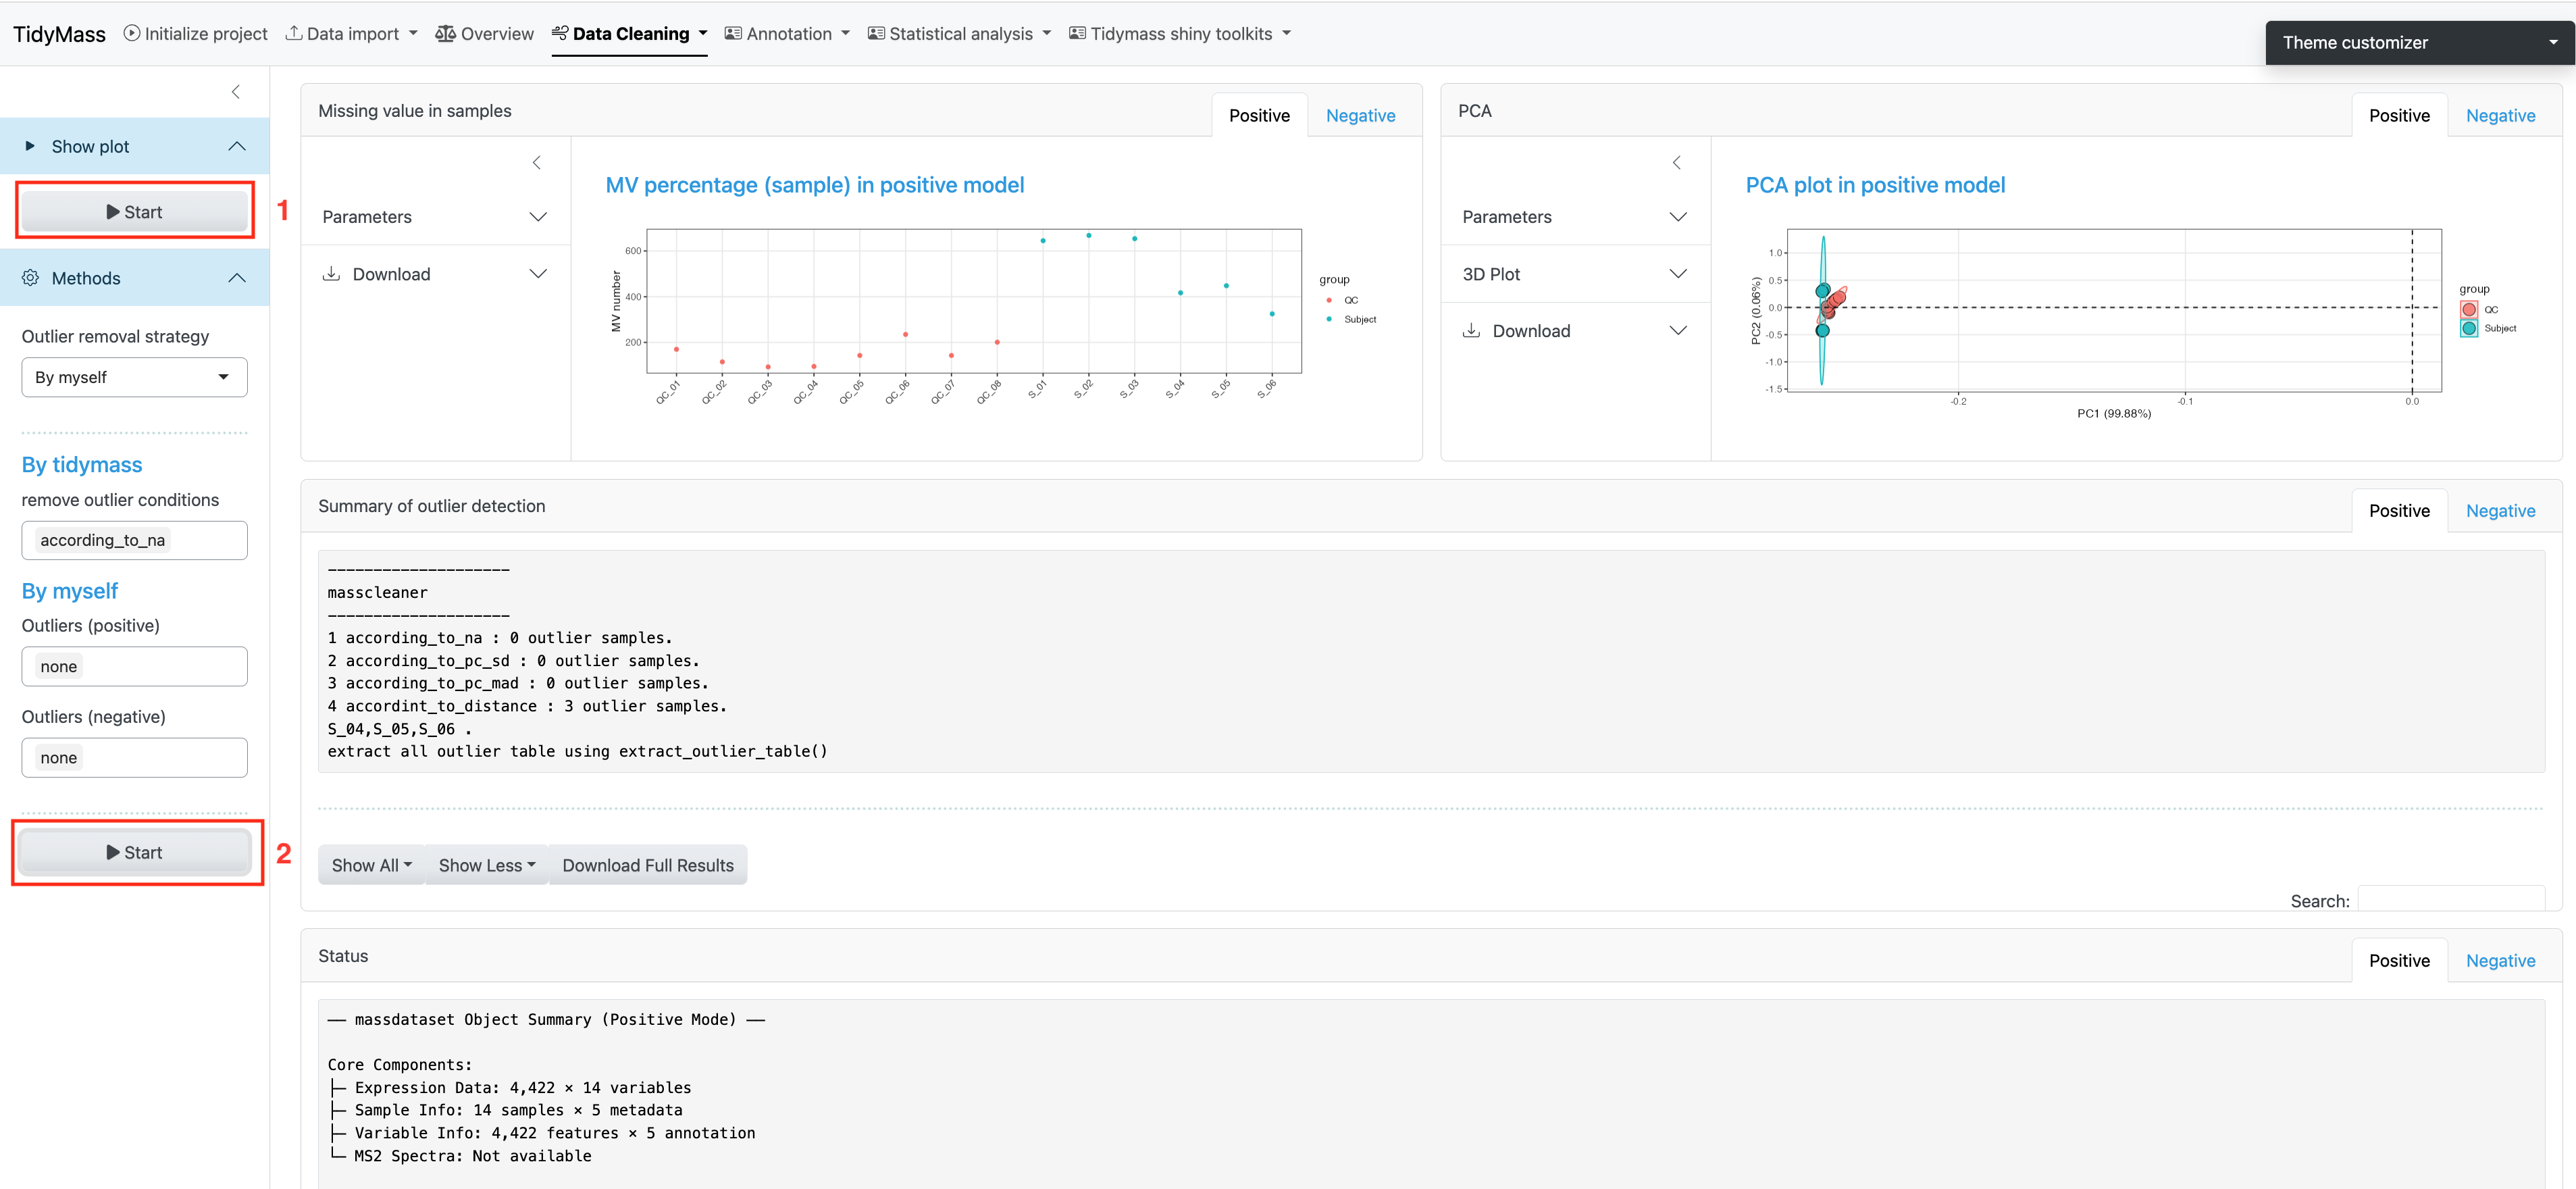
\includegraphics{figures/outliers.png}

In Tidymass shinyapp, we provide multiple options to filter outliers, you may select different strategies according to your requirement. For more information, please refer to this \href{https://privefl.github.io/blog/detecting-outlier-samples-in-pca/}{blog}.

For ``By tidymass'' strategy, four remove outlier conditions are provided: according to NA (according\_to\_na), accoriding to standard deviation for principal component (pc\_sd), according to mean abosolute deviation for principal component (pc\_mad) and according to distance (according\_to\_distance).

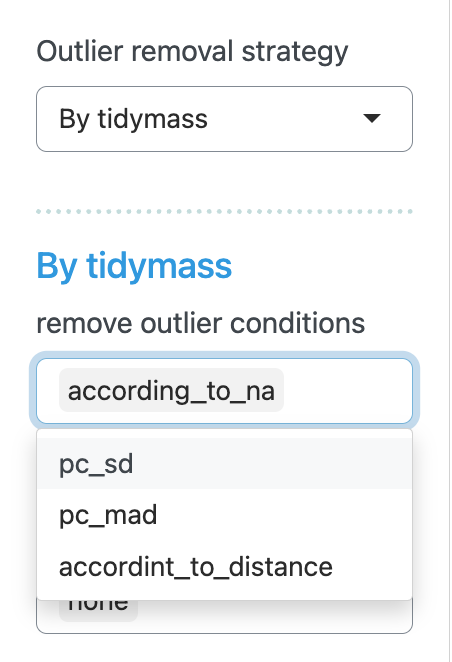
\includegraphics{figures/outliers_tidymass.png}

For ``By myself'' strategy, the outliers for both positive and negative modes are set to be ``none''.

Click \textbf{Start} below to filter outlier samples.

\textbf{Missing value imputation}

Here you can select many different methods for missing value imputation, including knn, missforest (mf) and ppca etc.

\textbf{Parameters}

For knn

\begin{itemize}
\tightlist
\item
  k: the parameters can be modified include number of neighbors. Defaults to 10.
\item
  rowmax: maximum row missing proportion. Defaults to 0.5.
\item
  colmax: maximum column missing proportion. Defaults to 0.8.
\item
  maxp: maximum prediction proportion. Defaults to 1500.
\item
  rng.seed: random number generator seed.
\end{itemize}

For missForest (rf)

\begin{itemize}
\tightlist
\item
  maxiter: the parameters include maximum iterations. Defaults to 10.
\item
  ntree: number of trees. Defaults to 100.
\item
  decreasing: whether to interpolate missing values in order from most to least number of missing values. Defaults to FALSE.
\end{itemize}

For ppca

\begin{itemize}
\tightlist
\item
  nPcs: the parameters can be modified include number of principal components. Defaults to 2.
\item
  maxSteps: maximum steps for iterations. Defaults to 100.
\item
  threshold: convergence threshold. Defaults to 1e-04.
\end{itemize}

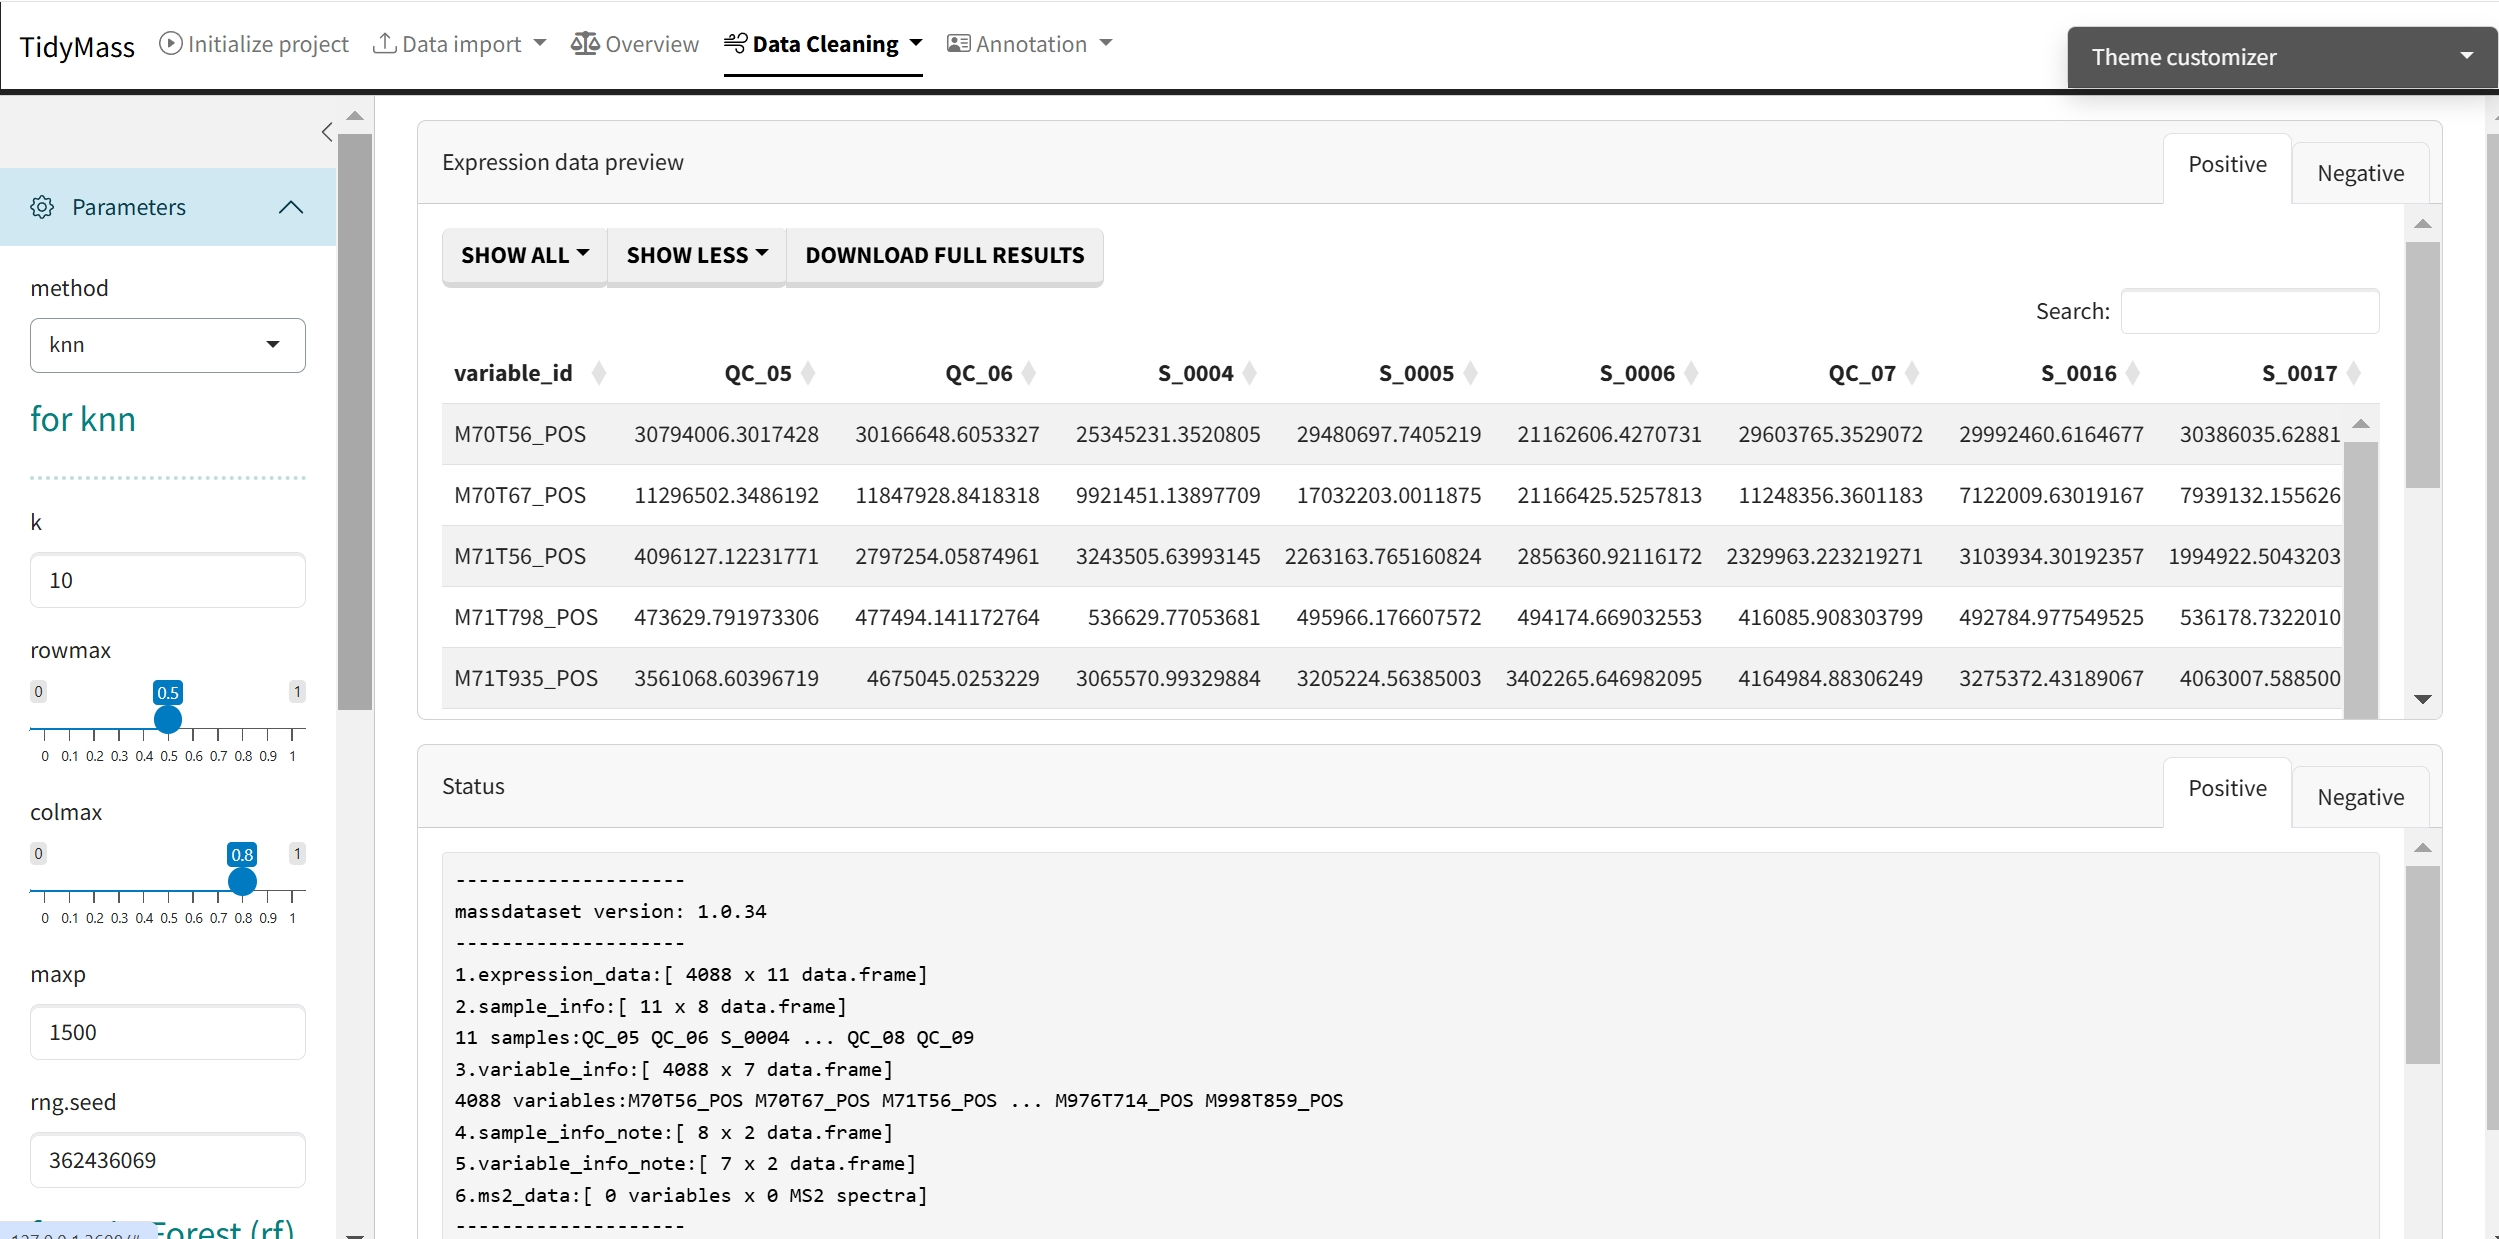
\includegraphics{figures/imputation1.png}

If the method has been chosen and all the parameters have been set, click \textbf{START} to perform missing value imputation.

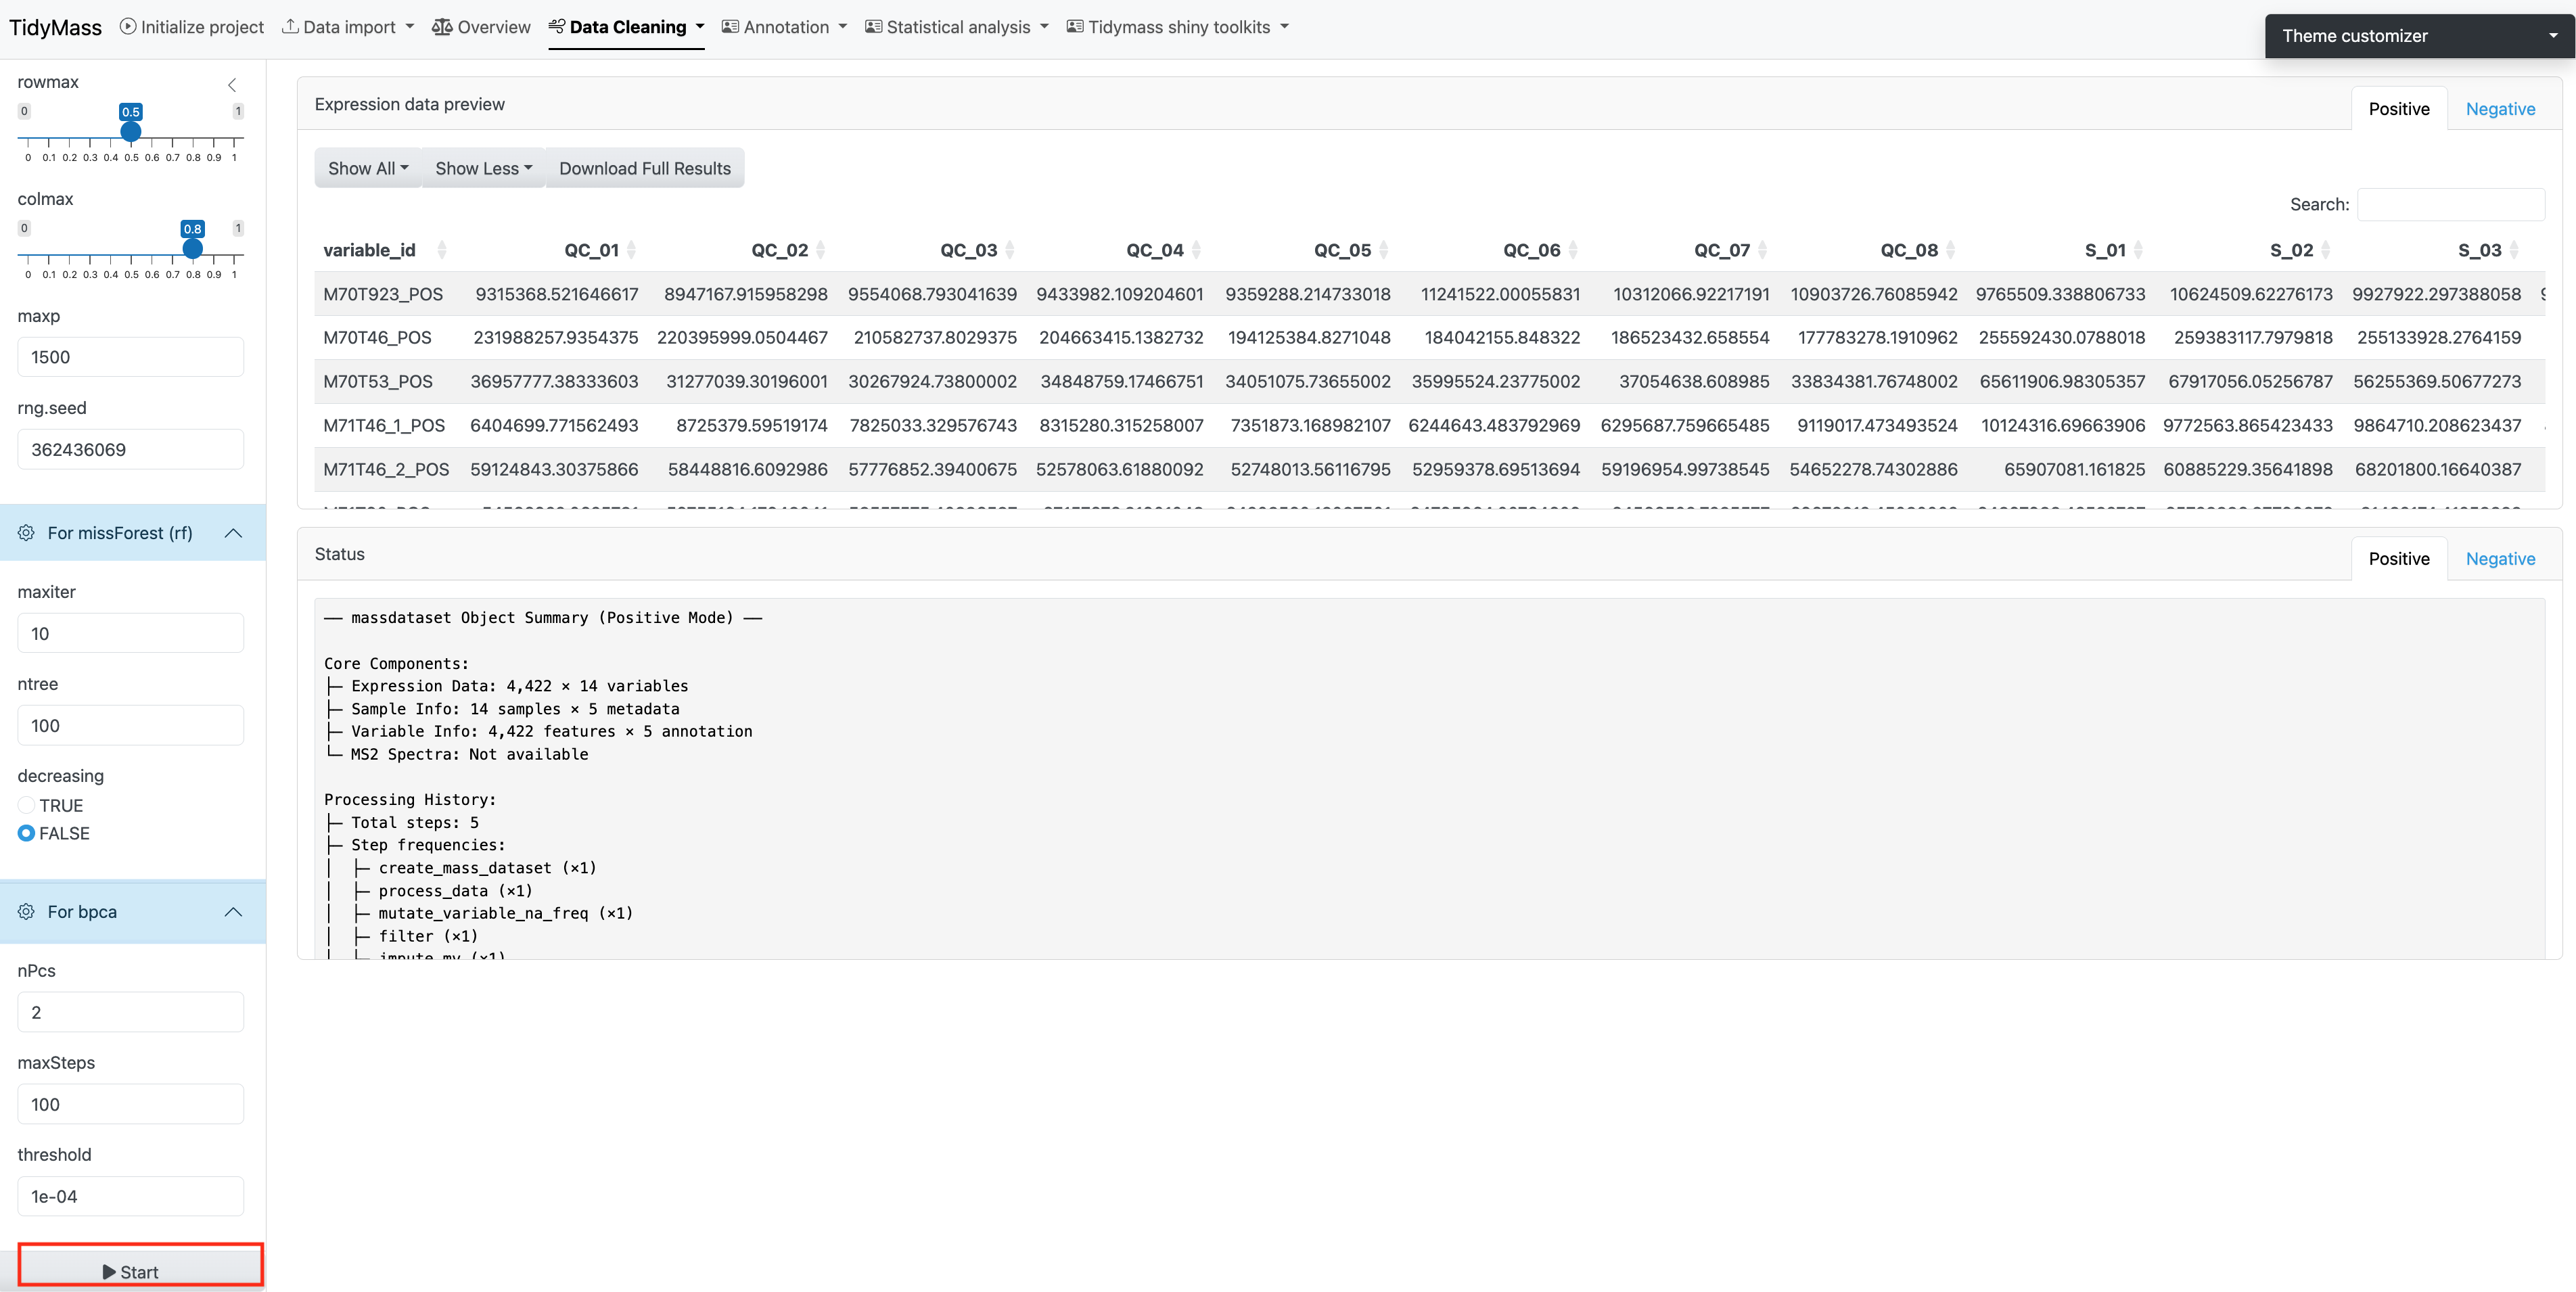
\includegraphics{figures/imputation2.png}

\textbf{Data normalization and integration}

To remove unwanted analytical variations and integrate multiple batches forming an integral data set for subsequent statistical analysis, we need to perform data normalization and integration.

Here we provide several methods to be selected, including QC sample-based data normalization like \texttt{svr} and \texttt{loess} and sample-wise method like \texttt{pqn}, \texttt{median}, \texttt{mean} and \texttt{total} intensity normalization.

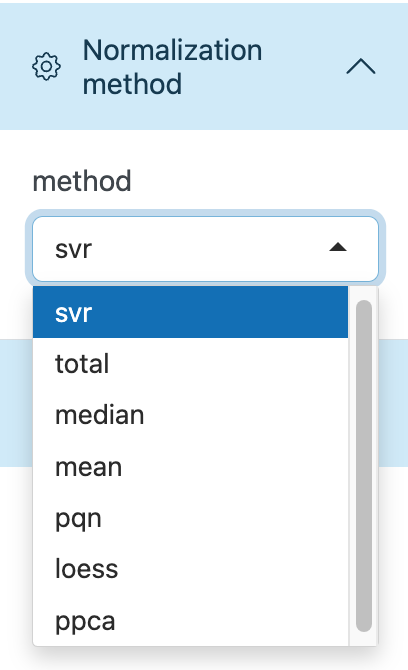
\includegraphics{figures/normalization_methods.png}

\textbf{Parameters}

\begin{itemize}
\tightlist
\item
  keep\_scale: whether to keep the original scale of the data during the data standardization process. Defaults to TRUE.
\item
  optimization: whether to enable optimization steps in the standardization process. Defaults to TRUE.
\item
  pqn\_reference: the reference value selected for using the Probabilistic Quotient Normalization method. Defaults to median.
\item
  begin\_value: the start value for parameter search range. Defaults to 0.5.
\item
  end\_value: the end value for parameter search range. Defaults to 1.
\item
  step\_value: the increment at each step of the parameter search. Defaults to 0.2.
\item
  multiple: the standardized factors used to control multiples. Defaults to 1.
\item
  threads: the number of threads for normalization. Defaults to 1.
\end{itemize}

Click \textbf{Start analysis} to perform the normalization and integration (The step may take some time, please be patient). Then click \textbf{Show plot} to visualize the difference before and after the normalization.

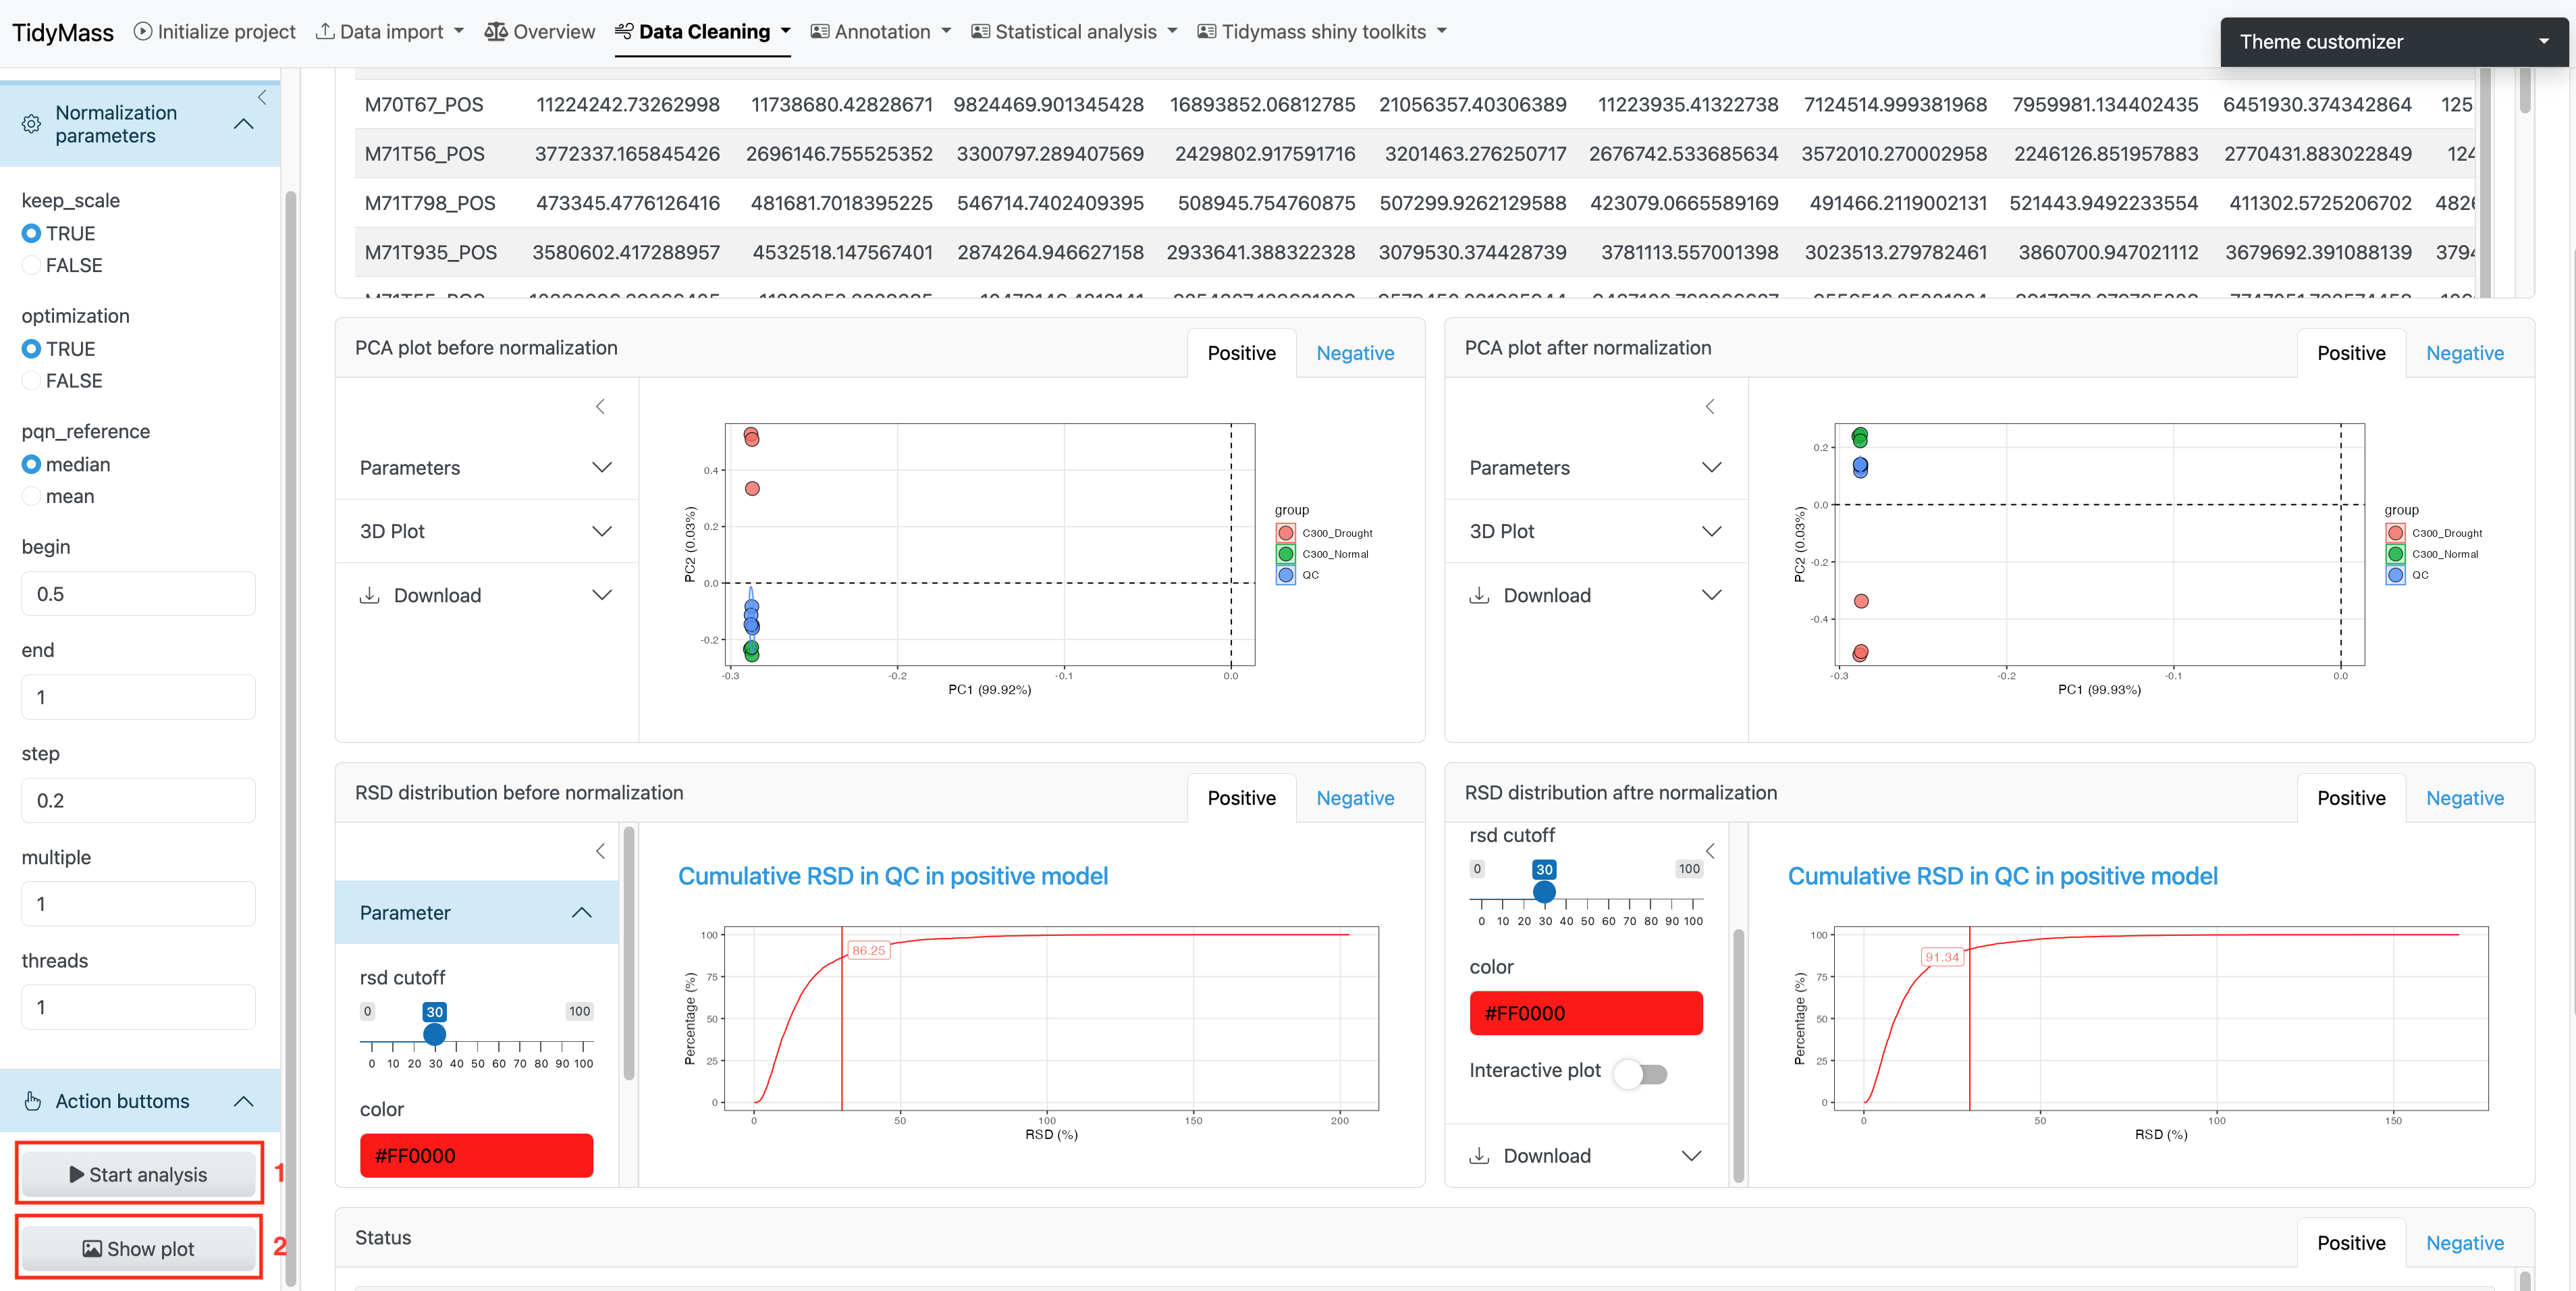
\includegraphics{figures/normaliztion.png}

\chapter{Downstream data processing}\label{downstream-data-processing}

\section{Metabolite annotation}\label{metabolite-annotation}

Metabolite annotation can be performed based on in-house and available open-source databases. To begin with, you need to click \textbf{Select MS2 folder} and import prepared MS2 data. These files should be in the format of ``.mgf'', and they should be stored separately for negative and positive modes.

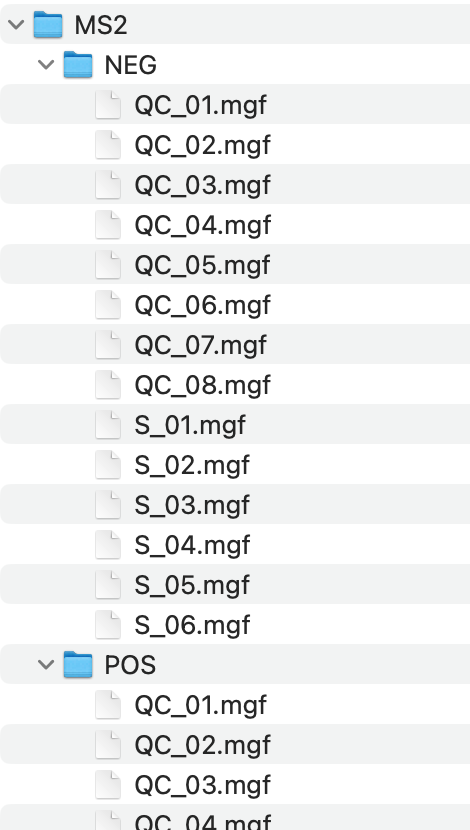
\includegraphics{figures/ms2_folder.png}

\textbf{Parameters}

\begin{itemize}
\tightlist
\item
  column: A character vector specifying the column types. Default is ``rp''.
\item
  ms1.ms2.match.mz.tol: Numeric, the m/z tolerance for matching MS1 and MS2. Default is 15.
\item
  ms1.ms2.match.rt.tol: Numeric, the retention time tolerance for matching MS1 and MS2. Default is 30.
\end{itemize}

Once you have set the parameters, click \textbf{Start} to import MS2 data.

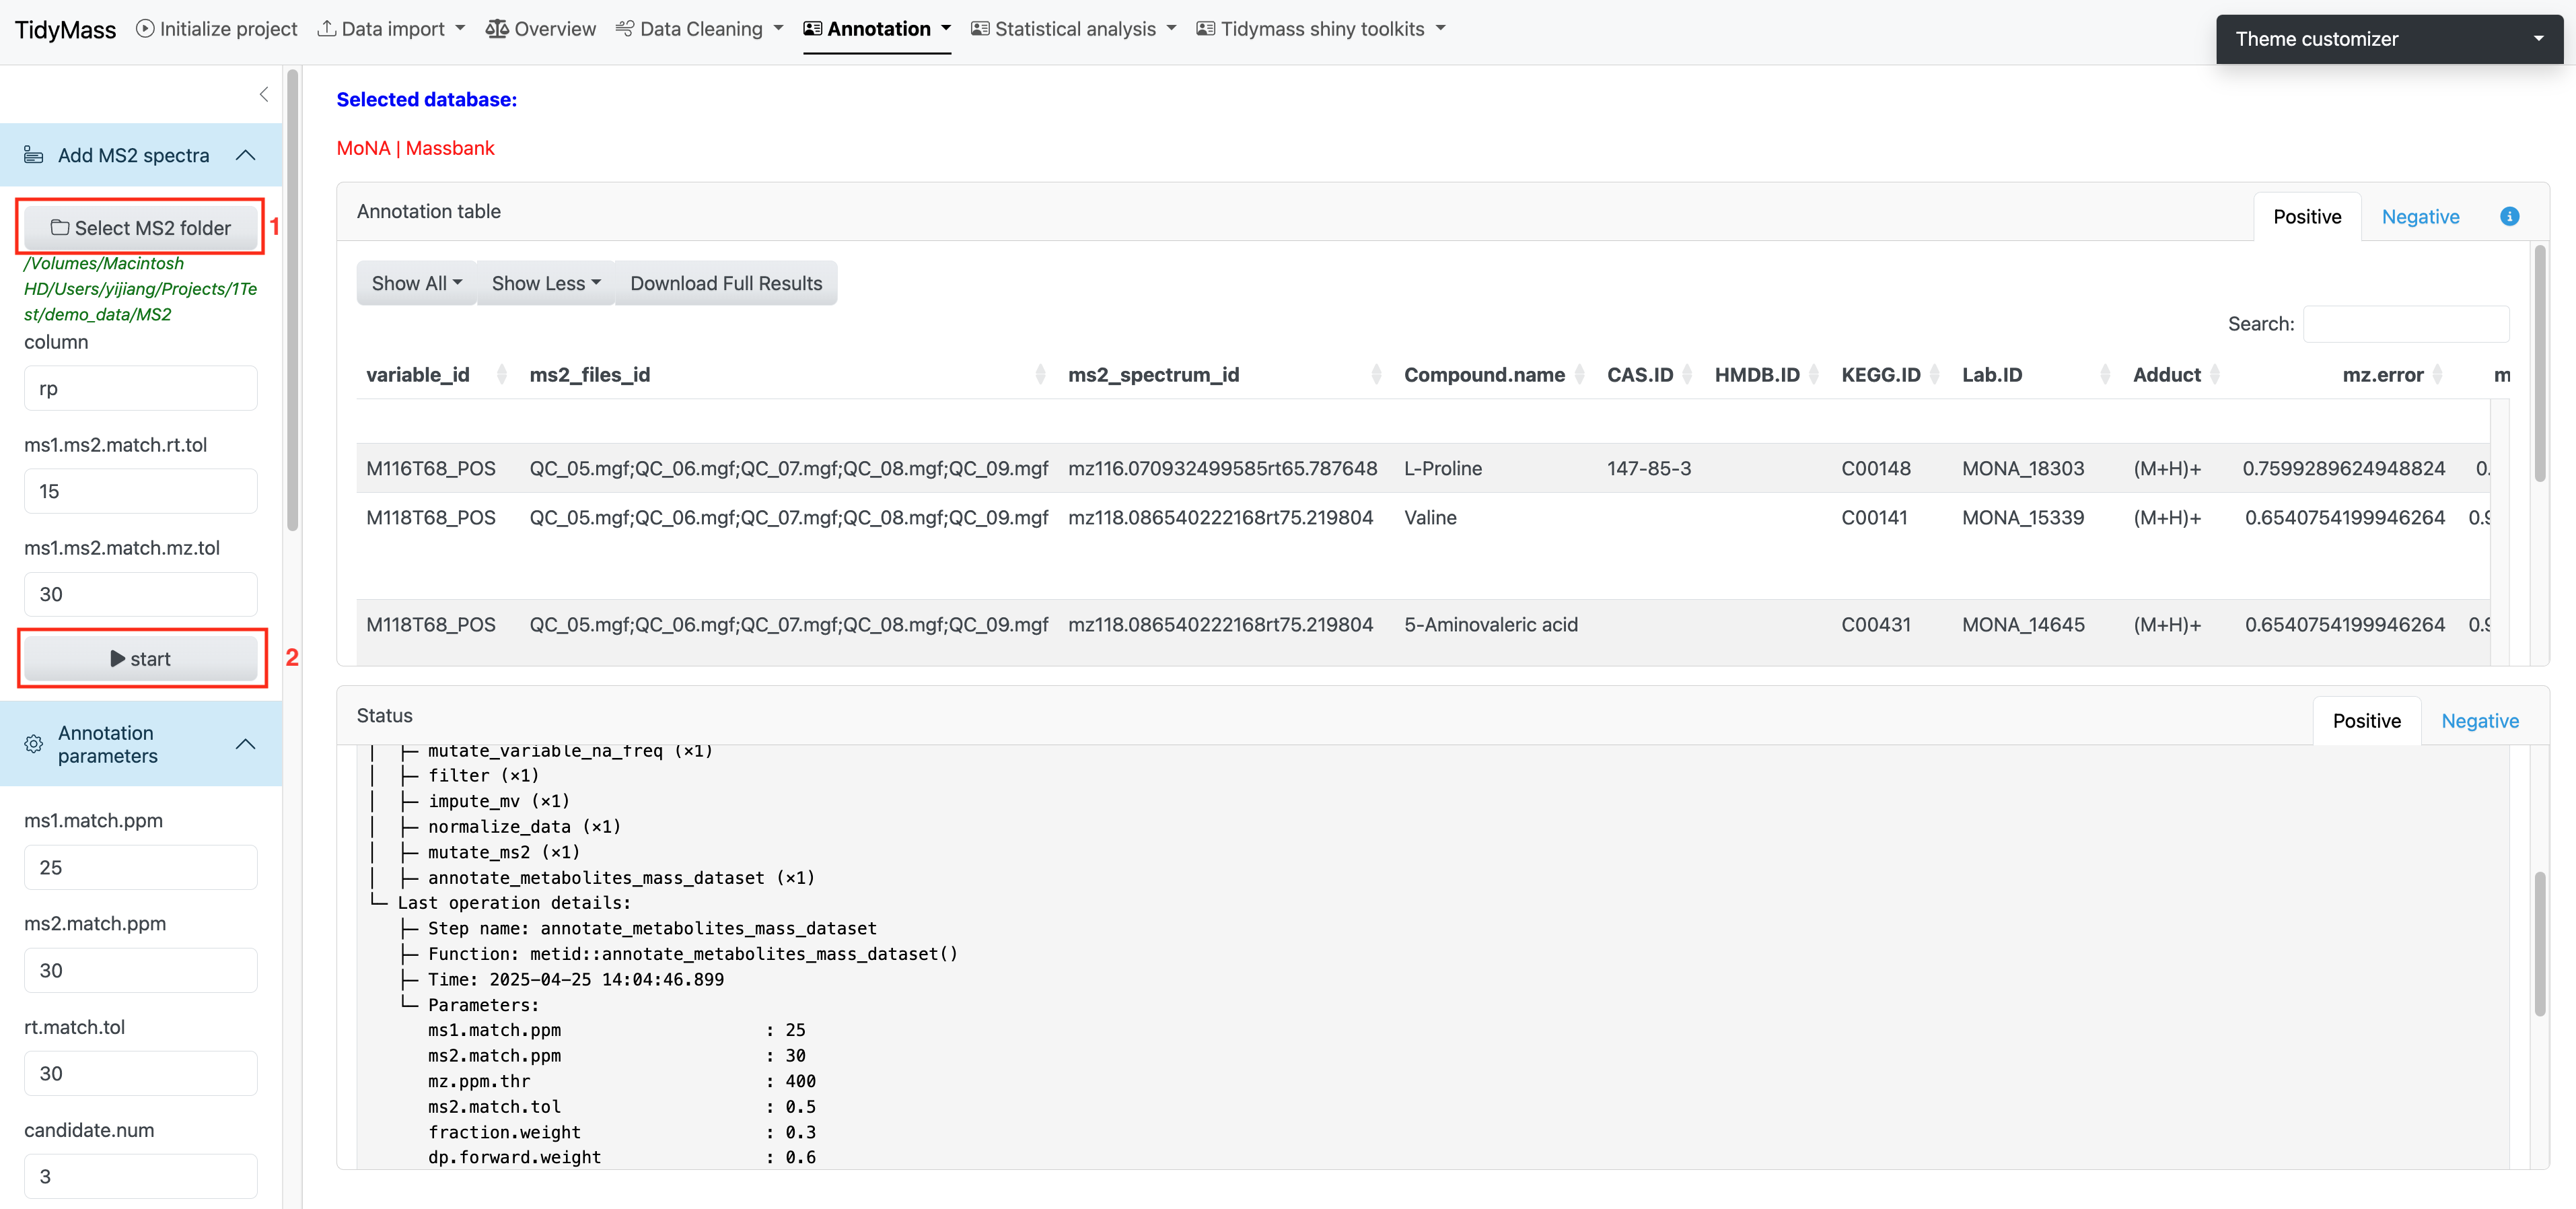
\includegraphics{figures/metabolite_annotation.png}

Next, you can choose suitable parameters for metabolite annotation.

\textbf{Parameters}

\begin{itemize}
\tightlist
\item
  ms1.match.ppm: A numeric value specifying the mass accuracy threshold for MS1 matching in parts per million (ppm). Defaults to 25.
\item
  ms2.match.ppm: A numeric value specifying the mass accuracy threshold for MS2 (Fragment ion) matching in ppm. Defaults to 30.
\item
  rt.match.tol: A numeric value specifying the retention time matching tolerance in seconds. Defaults to 30.
\item
  candidate.num: A numeric value specifying the number of top candidates to retain per feature. Defaults to 3.
\item
  column: A character string specifying the chromatographic column type, either ``rp'' (reverse phase) or ``hilic''. Defaults to ``rp''.
\item
  threads: An integer specifying the number of threads to use for parallel processing. Defaults to 3.
\end{itemize}

We need necessary MS2 databases for metabolite annotation, and here we provide some common in-house databases.

More MS2 compound databases can be downloaded from \href{https://www.tidymass.org/databases/}{Tidymass Website}. After the download is complete, place them in a new folder and click \textbf{Choose folder}.

You can also use Tidymass to build your own database, please be noted that the format should be in ``.rda''.

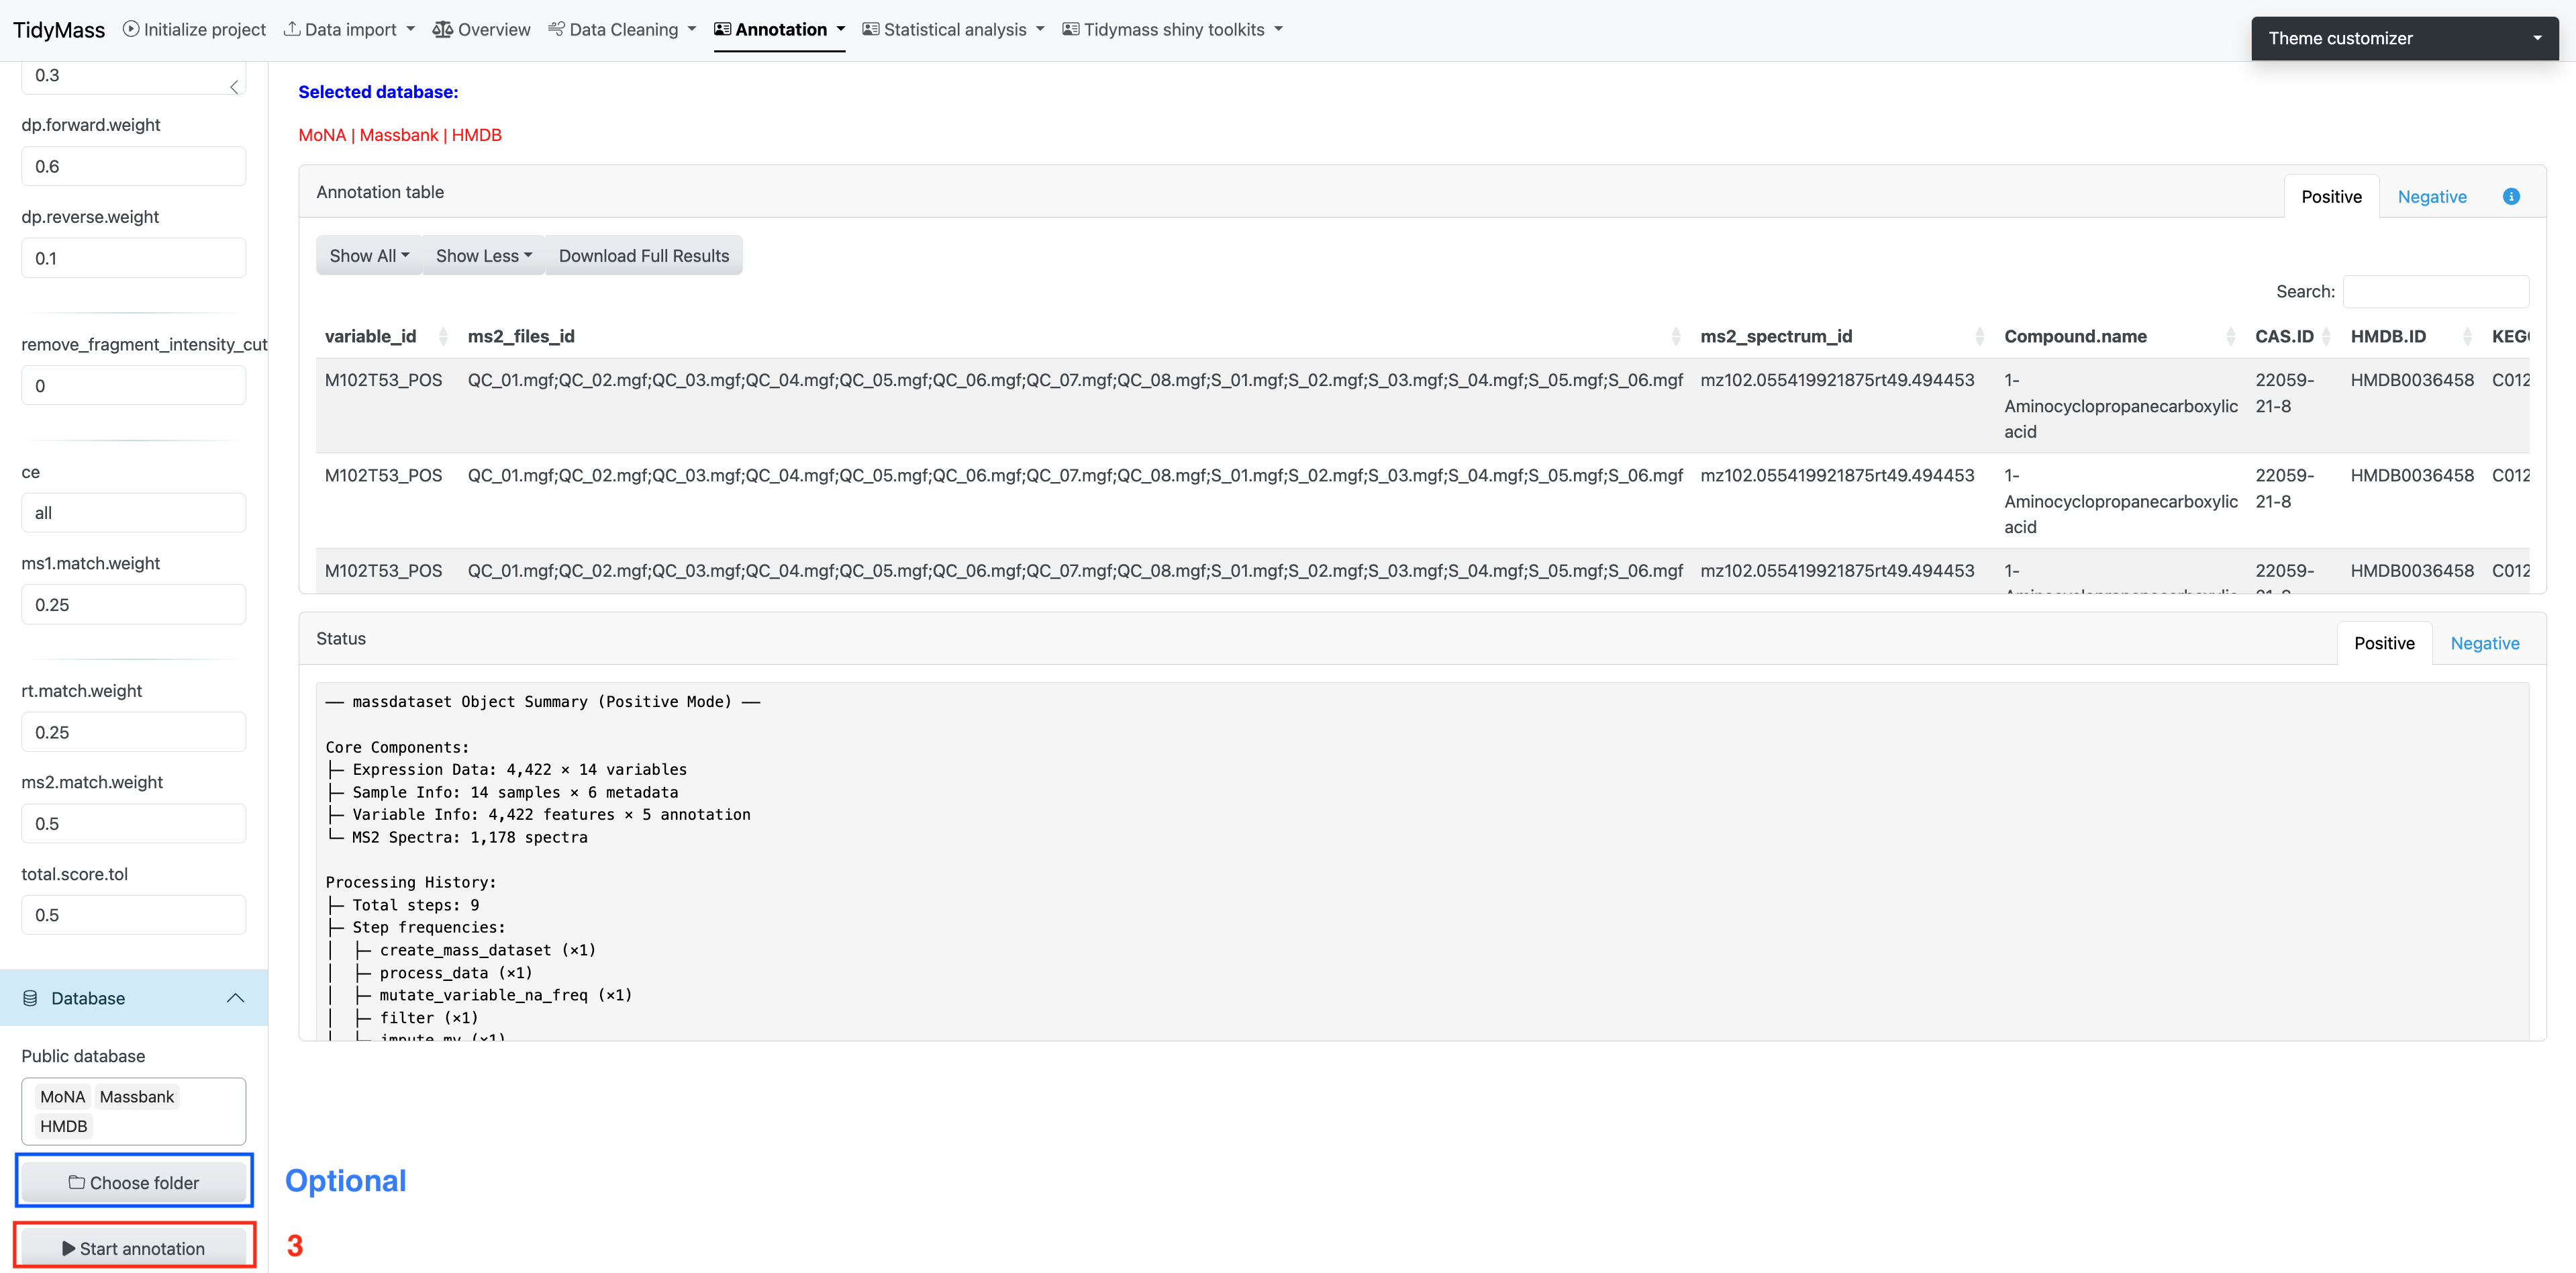
\includegraphics{figures/metabolite_annotation2.png}

\section{Annotation filtering}\label{annotation-filtering}

The annotation results are assigned confidence levels according to MSI (in-house database, level 1; public MS2 database, level 2; MS1 database, level 3).

After obtaining annotation results, you can choose how to keep multiple annotations, how to remove redundancy and how to keep annotation levels.

Click \textbf{Adduct for level 3 annotation} and select suitable models and methods, then click \textbf{START} to perform annotation filtering.

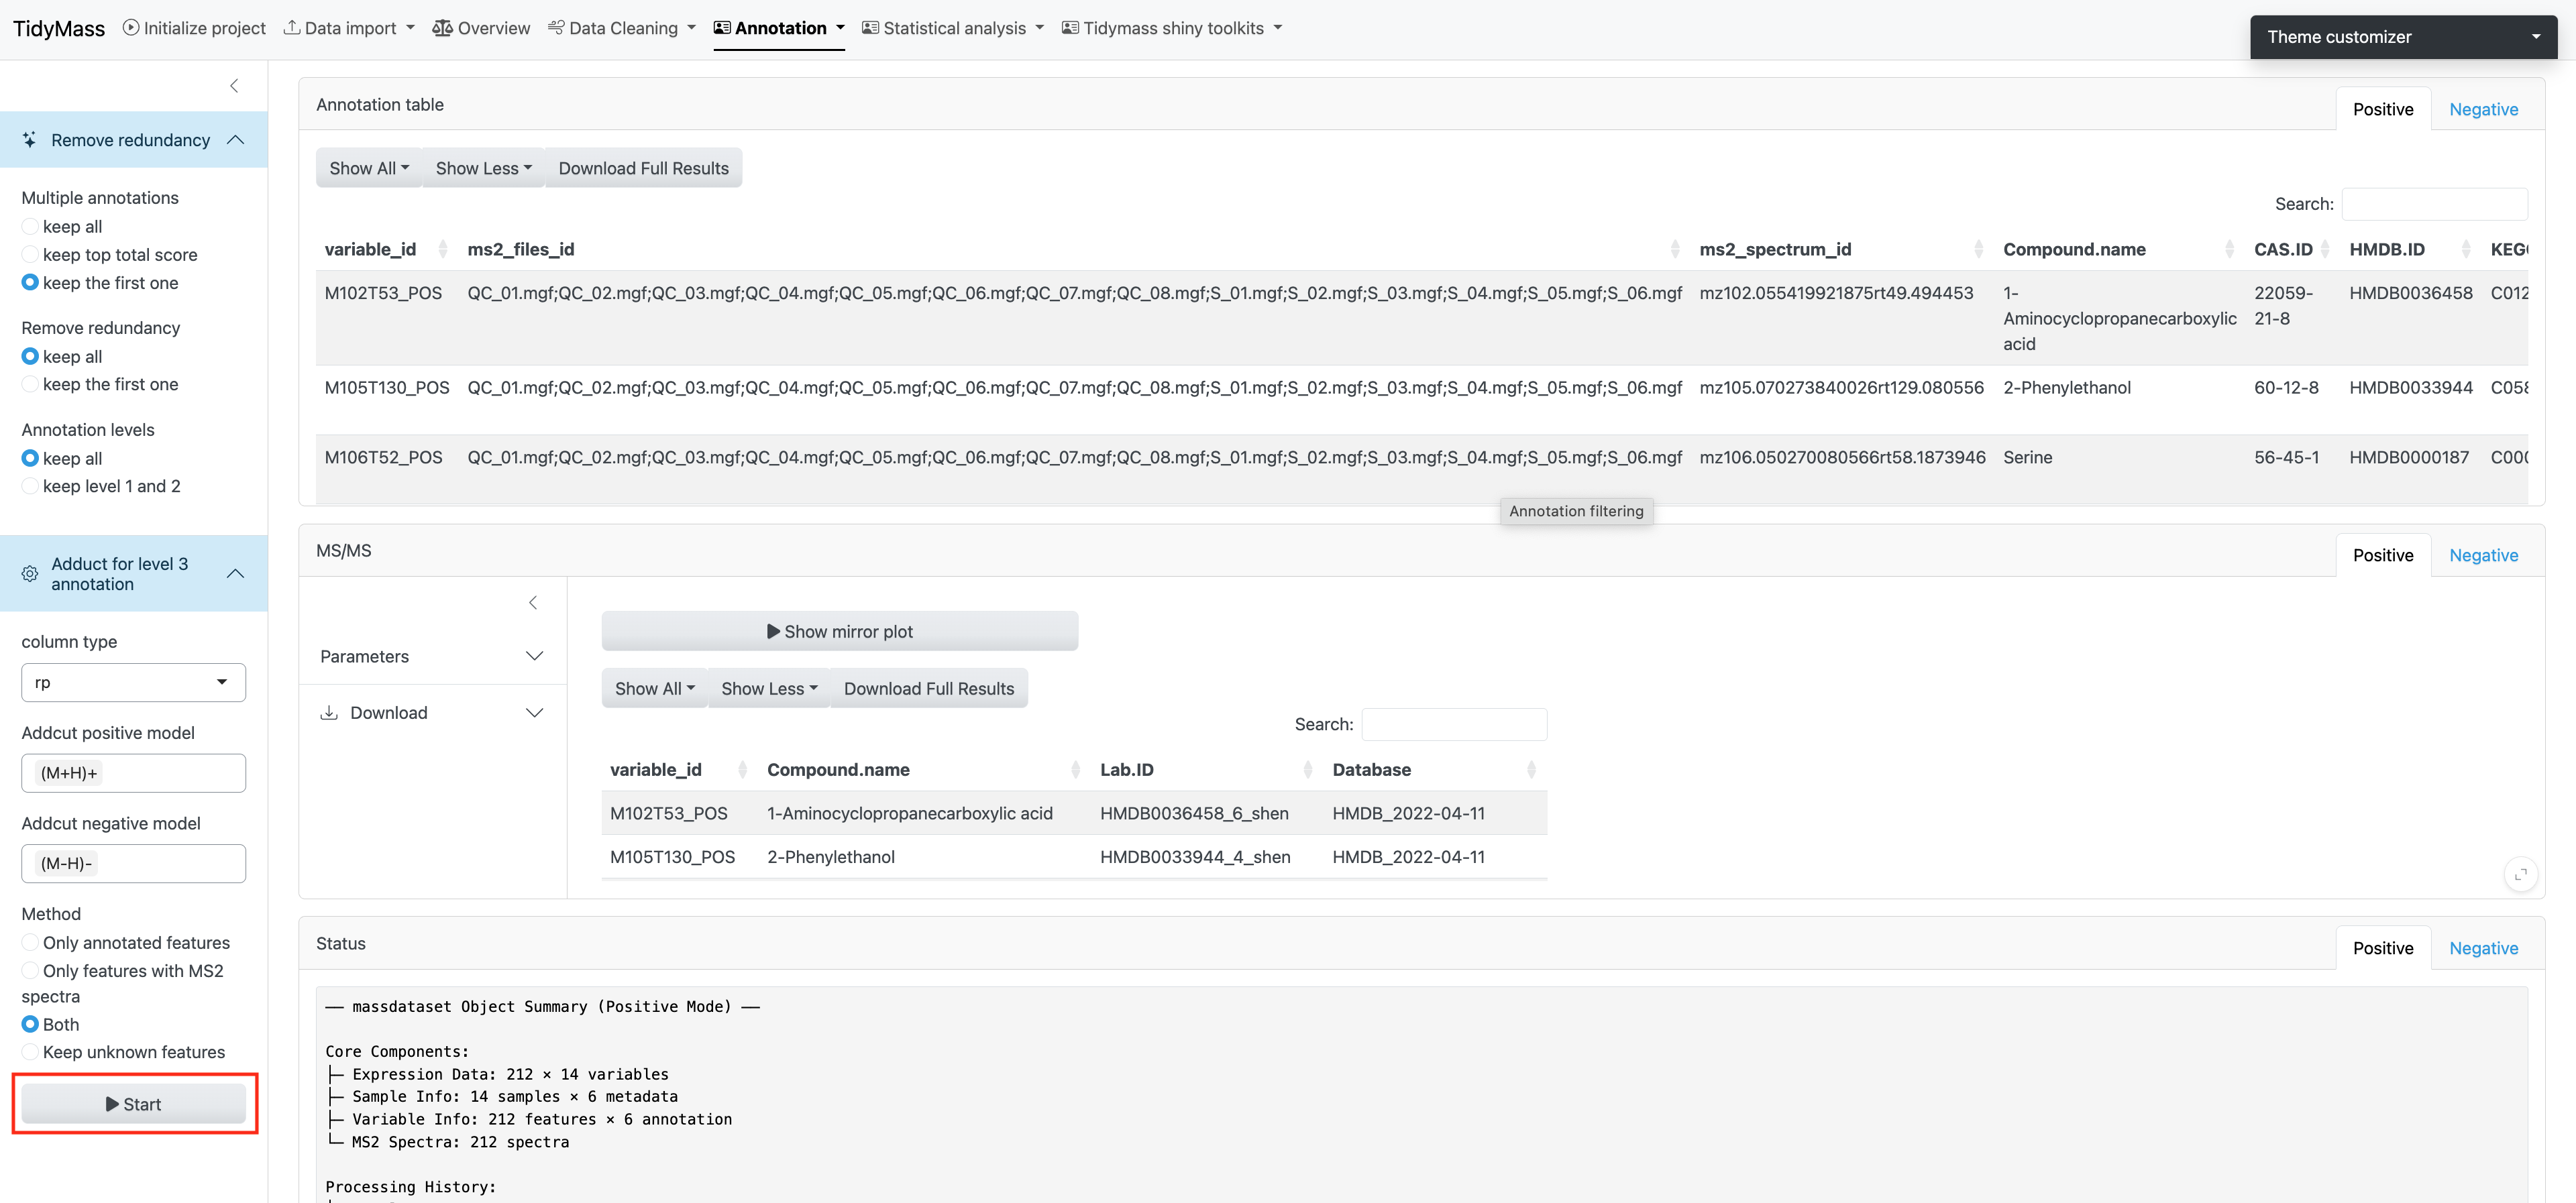
\includegraphics{figures/annotation_filtering.png}

\section{Merge data}\label{merge-data}

\section{Differential Accumulated Metabolites (DAM)}\label{differential-accumulated-metabolites-dam}

\section{Enrichment}\label{enrichment}

\section{Feature-based Pathway Analysis (FPA)}\label{feature-based-pathway-analysis-fpa}

\chapter{References}\label{references}

\begin{enumerate}
\def\labelenumi{\arabic{enumi}.}
\tightlist
\item
  Shen, X., Yan, H., Wang, C. et al.~TidyMass an object-oriented reproducible analysis framework for LC--MS data. Nat Commun 13, 4365 (2022). \url{https://doi.org/10.1038/s41467-022-32155-w}
\item
  \url{https://www.tidymass.org/}
\item
  \url{https://github.com/tidymass/tidymass_shiny}
\end{enumerate}

  \bibliography{book.bib,packages.bib}

\end{document}
